\documentclass[xcolor={dvipsnames}]{beamer}

\usepackage[utf8]{inputenc}
\usetheme{default}
\usepackage[scaled=0.85]{helvet}
% \usepackage[dvipsnames]{xcolor}
% \addtobeamertemplate{footline}{\insertframenumber/\inserttotalframenumber}
\usepackage{epsfig}
\usepackage{tikz}
\usepackage{multicol}
\usepackage{caption}

\newcommand{\centered}[1]{\begin{tabular}{l} #1 \end{tabular}}

\definecolor{bleu}{rgb}{0.2,0.2,0.7}

\title{Modélisation du système manguier -- cécidomyies des fleurs pour une évaluation de modes de gestion du ravageur et de ses dégâts}
\date{}
\author{}

\setbeamertemplate{footline}{
% \small
\hspace{12cm}\insertframenumber{} / \inserttotalframenumber{}
\vspace{0.15cm}
}
\setbeamertemplate{caption}[numbered]

\begin{document}

%% TITRE
\begin{frame}



%  \maketitle
\begin{center}
 {\color{bleu} \Large Modélisation du système manguier – cécidomyies
des fleurs pour une évaluation de modes de gestion
du ravageur et de ses dégâts}
\vspace{0.5cm}

Bastien Reyné
\end{center}

 \begin{center}
 
\includegraphics[scale = 0.35]{um.pdf}
 \hspace{0.8cm}
 
\epsfig{file = ../plots/logo_cirad2.eps, scale = 0.09}
 \end{center}
 

{\small \begin{tabular}{lll}
{Encadrants} & Isabelle Grechi & UPR HortSys\\
 & Frédéric Boudon & équipe M2P2 (UMR AGAP)\\
% Responsables pédagogiques & Xavier Bry & FDS\\
%  & Corinne Janicot & IAE
 \end{tabular}
}
 \vspace{0.5cm}
 
{\small \begin{tabular}{lll}
% Encadrants & Isabelle Grechi & Cirad, UPR HortSys\\
%  & Frédéric Boudon & Cirad, équipe M2P2 (UMR AGAP)\\
Responsables pédagogiques & Xavier Bry & FDS\\
 & Corinne Janicot & IAE
 \end{tabular}
} 
\end{frame}










%% PROBLÉMATIQUE
\begin{frame}
 \frametitle{Problématique}
 
 
 
 \begin{multicols}{2}
 Le manguier est arbre fruitier qui présente de forts asynchronismes phénologiques.

 \vspace{0.2cm}
 
 $\rightarrow$ Favorise la prolifération des ravageurs

 \begin{figure}
 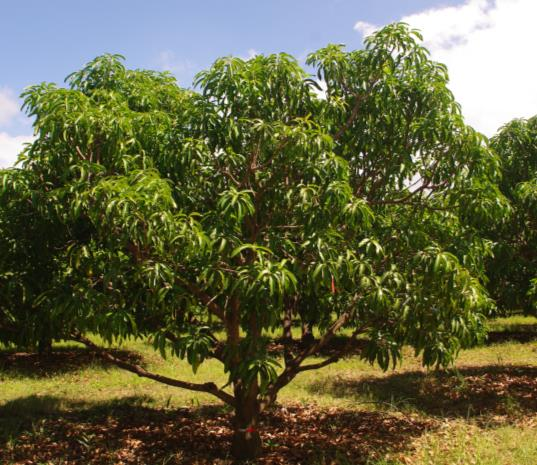
\includegraphics[scale = 0.37]{manguier.jpg}
{\scriptsize \caption{Un manguier \footnote{photos : I. Grechi, A. Franck}}}
 \end{figure}
\end{multicols}

\pause

 \begin{multicols}{2}
 La cécidomyie des fleurs

 \vspace{0.2cm}
 
 $\rightarrow$ S'attaque aux inflorescences

 \begin{figure}
 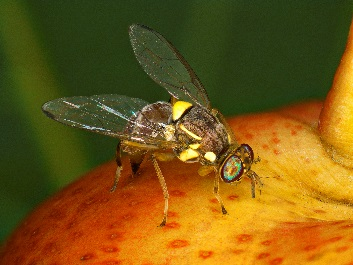
\includegraphics[scale = 0.8]{cecido.jpg}
\caption{Une cécidomyie des fleurs\footnote{photo : A. Franck}}
 \end{figure}

 
\end{multicols}
 
\end{frame}


%% OBJECTIFS
\begin{frame}
 \frametitle{Objectif}
 
 Établir un modèle décrivant la dynamique de population de cécidomyies des fleurs en fonction de la dynamique de population d'inflorescences.
 
 \vspace{1cm}
 
$\longrightarrow$ Améliorer la compréhension du système manguier -- cécidomyies
\end{frame}



%% CONNAISSANCES MANGUIERS
\begin{frame}
 \frametitle{Connaissances}
 \begin{figure}[ht]
 \centering
 \begin{columns}
        \column{.3\linewidth}
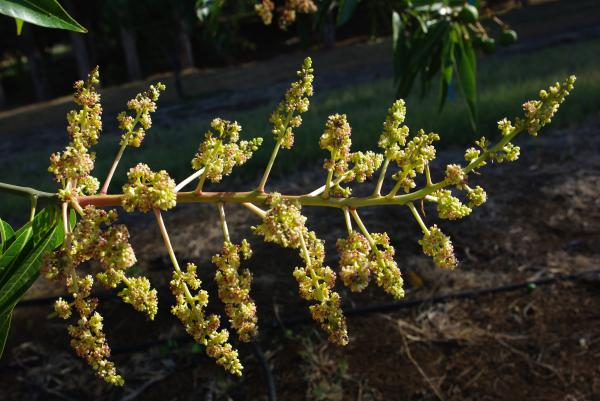
\includegraphics[scale = 0.29]{../photos/inflo3.jpg}
        \column{.4\linewidth}
 \caption{Une inflorescence de manguier (photo : F. Normand)}
        \label{fig:inflos}
  \end{columns}
%  \includegraphics[bb=0 0 3872 2592,scale=0.079]{photos/inflo.jpg}

 % inflo.jpg: 3872x2592 px, 72dpi, 136.60x91.44 cm, bb=0 0 3872 2592
 
 \label{fig:inflo}
\end{figure}
\begin{figure}[ht]
 \centering
 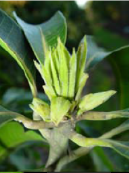
\includegraphics[scale = 0.5]{../photos/infloC.png}
 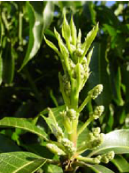
\includegraphics[scale = 0.5]{../photos/infloD.png}
 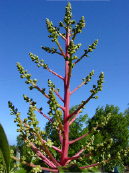
\includegraphics[scale = 0.5]{../photos/infloE.png}
 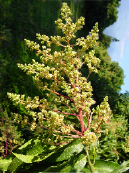
\includegraphics[scale = 0.5]{../photos/infloF.png}
 
 C \hspace{1.4cm} D \hspace{1.4cm} E \hspace{1.4cm} F
 % inflo.jpg: 3872x2592 px, 72dpi, 136.60x91.44 cm, bb=0 0 3872 2592
 \caption{Les stades phénologiques C à F d'une inflorescence de manguier (photos : F. Normand)}
 \label{fig:stades_inflo}
\end{figure}

\end{frame}


%% CONNAISSANCES CÉCIDOMYIES
\begin{frame}
 \frametitle{Connaissances}
 
 \begin{figure}
 \centering
 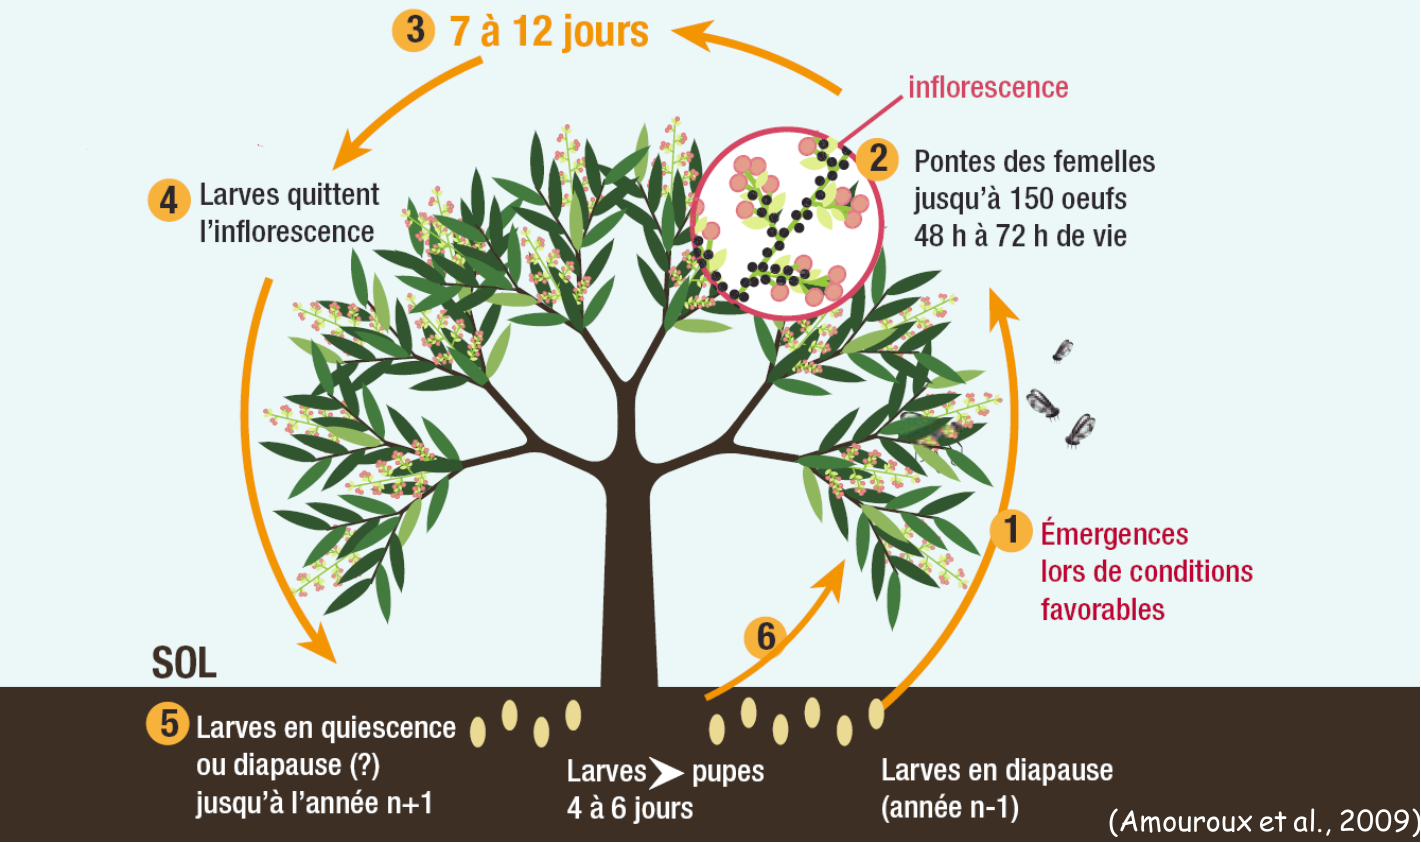
\includegraphics[scale = 0.2]{../photos/cycle.png}
%  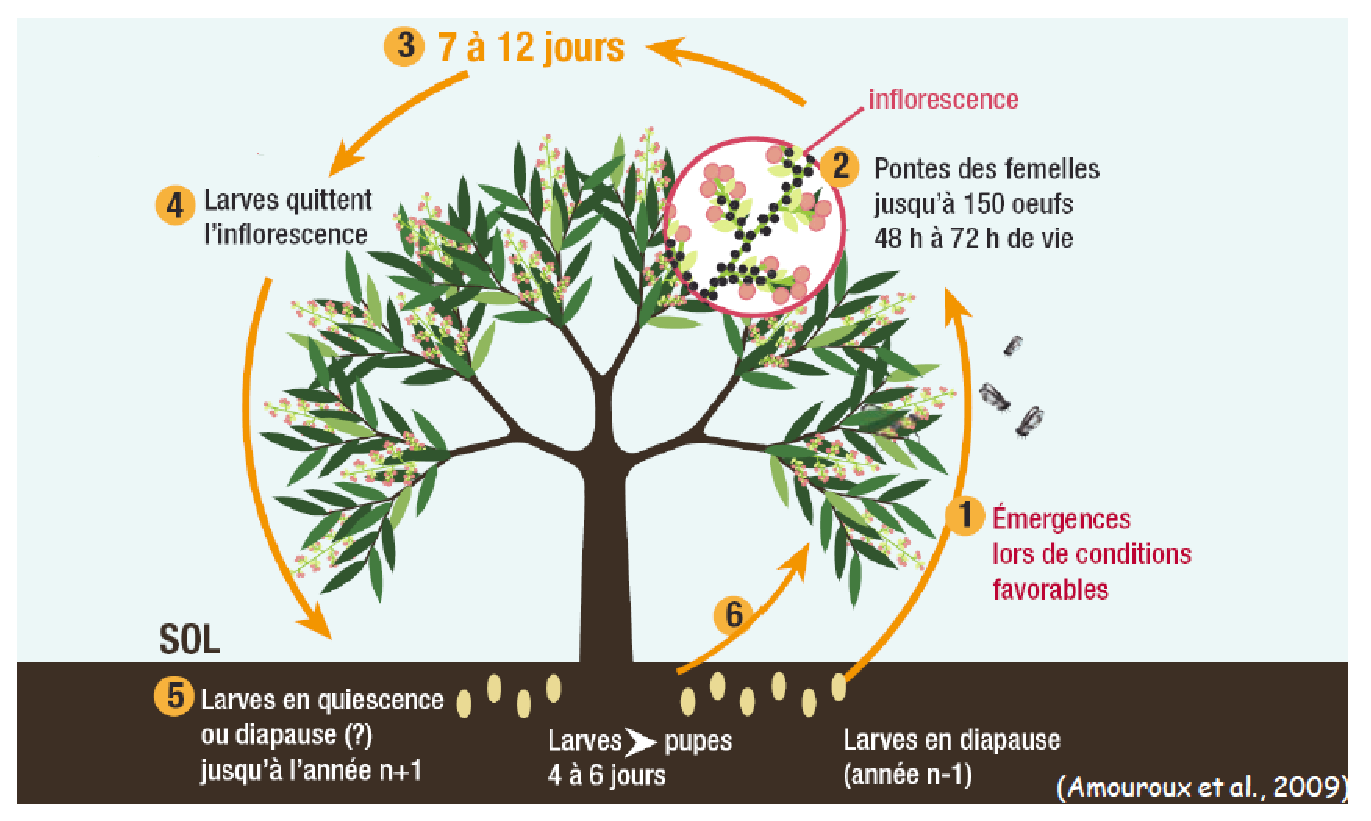
\epsfig{file = photos/cycle.eps, scale = 0.5}
 \caption{Représentation du cycle de développement de la cécidomyie des fleurs du manguier.}
 \label{fig:cycle}
\end{figure}
%
\end{frame}


\begin{frame}
 \frametitle{Expérimentation}
 \begin{figure}[ht]
 \centering
 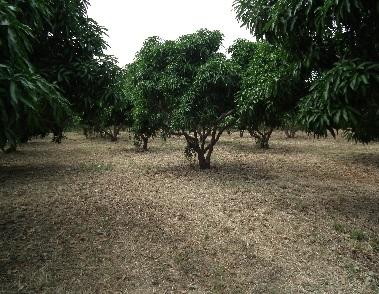
\includegraphics[scale = 0.5]{../photos/er.jpg}
 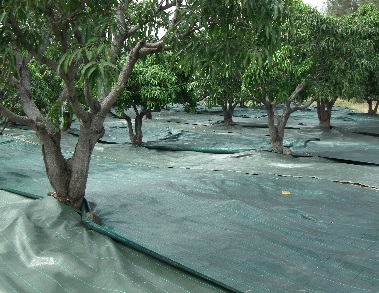
\includegraphics[scale = 0.5]{../photos/ps.jpg}
 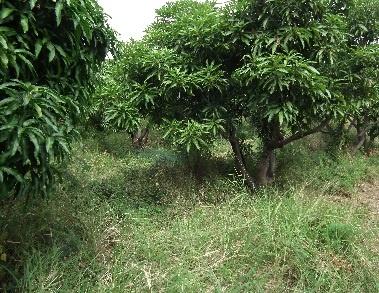
\includegraphics[scale = 0.5]{../photos/eh.jpg}
 
  \vspace{0.3cm}
 
 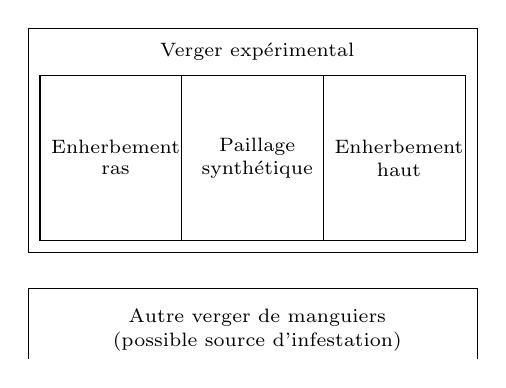
\begin{tikzpicture}[scale = 0.3]
  \draw (0,5) rectangle (18, 12);
  \draw (6, 5) -- (6, 12);
  \draw (12, 5) -- (12, 12);
  \draw (-0.5, 0) -- (-0.5, 3) ;
  \draw (-0.5, 3) -- (18.5, 3) ;
  \draw (18.5, 3) -- (18.5, 0);
  \draw (9, 1.75) node{\text{ \scriptsize Autre verger de manguiers}};
  \draw (9, 0.75) node{\text{ \scriptsize (possible source d'infestation)}};
  \draw (9, 9) node{\text{   \scriptsize Paillage}};
  \draw (9, 8) node{\text{    \scriptsize synthétique}};
  \draw (3, 9) node{\text{   \scriptsize Enherbement}};
  \draw (3, 8) node{\text{    \scriptsize ras}};
  \draw (15, 9) node{\text{  \scriptsize Enherbement}};
  \draw (15, 8) node{\text{   \scriptsize haut}};
  \draw (-0.5, 4.5) rectangle (18.5, 14);
  \draw (9, 13) node{\text{   \scriptsize Verger expérimental }};
 \end{tikzpicture}
 \caption{Description du dispositif mis en place sur les parcelles expérimentales}
 \label{fig:exp}
\end{figure}
\end{frame}







%% DATA
\begin{frame}
 \frametitle{Données disponibles}
 
 \begin{figure}

  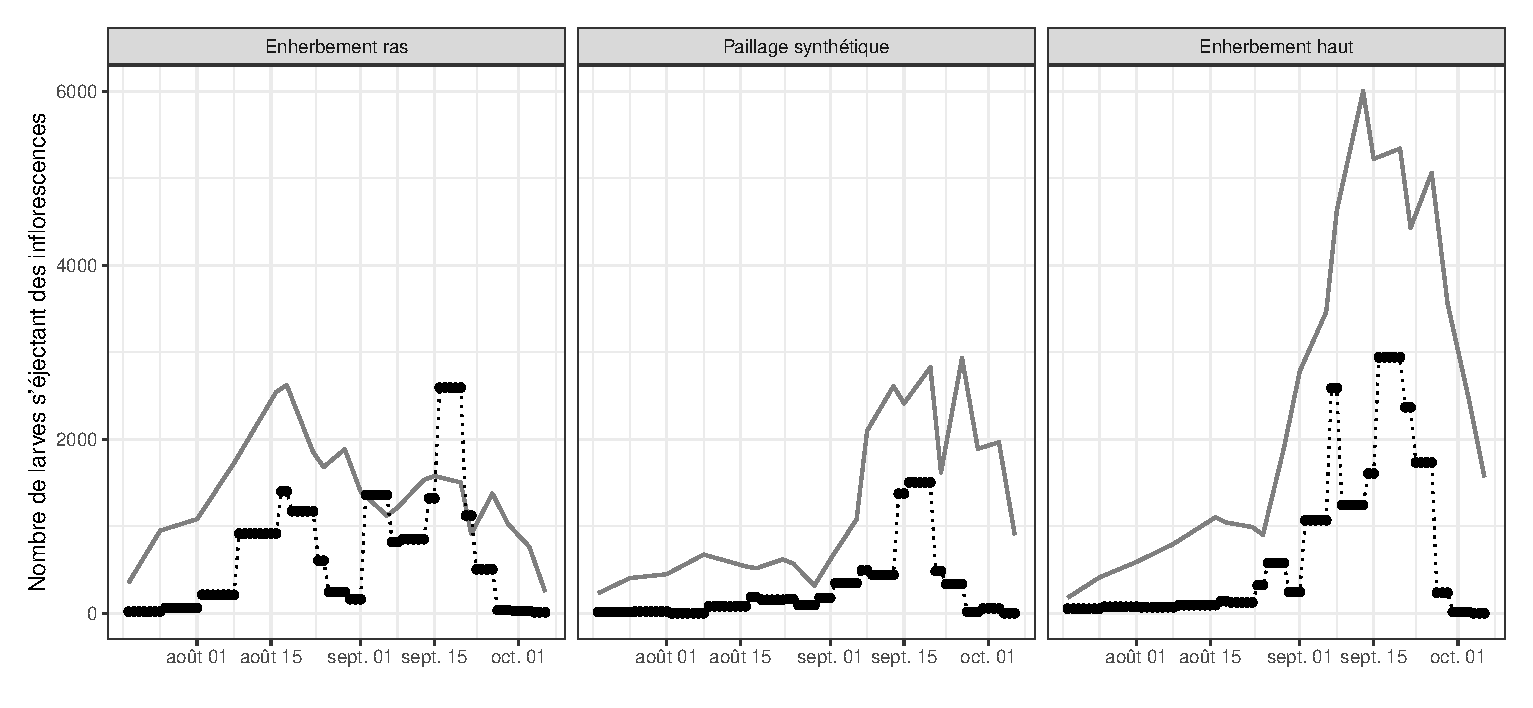
\epsfig{file = ../r/larves.eps, scale = 0.3}
  
  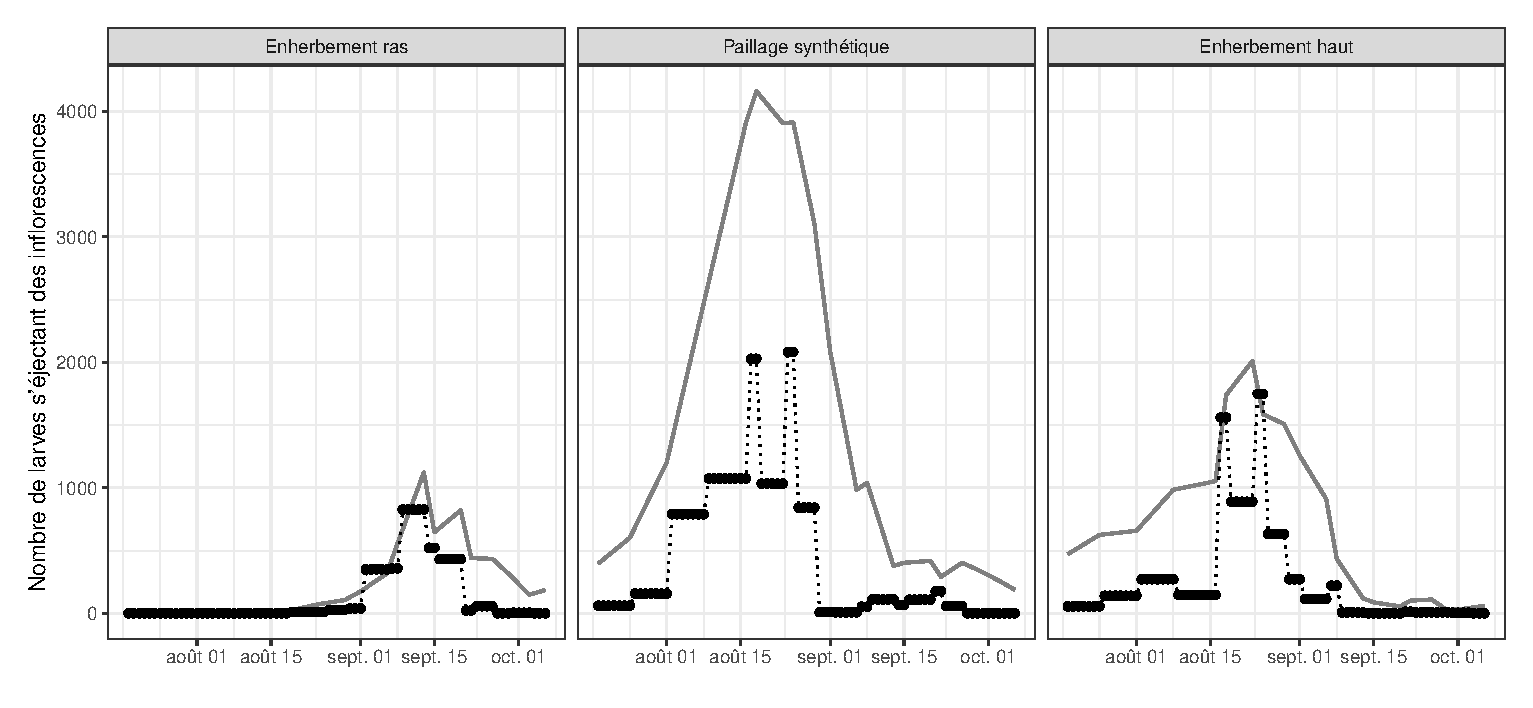
\epsfig{file = bloc2.eps, scale = 0.3}
  \caption{Dynamiques de larves et d'inflorescences pour chacun des deux vergers}
  \label{fig:l}
 \end{figure}

 
\end{frame}
















\begin{frame}
 \frametitle{Modèle}
 
 \textbf{Objectif : } Décrire la dynamique de population de cécidomyie des fleurs à l'intérieur d'un verger.
 
 \vspace{1cm}
 
 Entrée : Dynamiques d'inflorescences
 
 \vspace{1cm}
 
 Sortie : Dynamiques de cécidomyies (larves et adultes)
\end{frame}








%% MODÈLE

\begin{frame}
  \frametitle{Modèle}
 %% SCHÉMA
%  \only<1>{
\begin{figure}[ht]
  \centering
  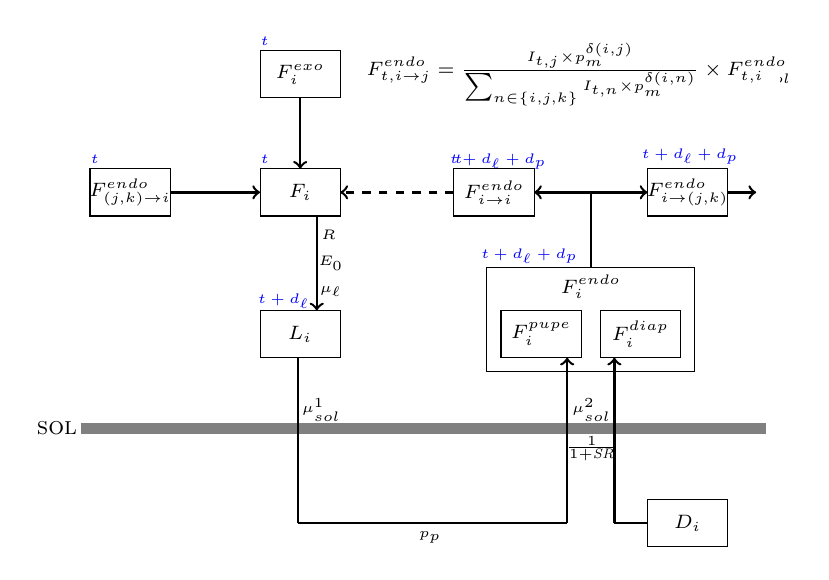
\begin{tikzpicture}[scale = 0.6]
\draw (0, 0) node{\small \textsc{sol}};
\draw [line width = 1.5mm, color = gray] (0.5, 0) -- (15, 0);
   
\draw (4.3,   4.5) rectangle (6, 5.5); % N
\draw (5.15,   5) node {\scriptsize $F_{i}$};
\draw (4.4, 5.7) node {\tiny $\textcolor{blue}{t}$};
\pause

\draw (4.3,   7) rectangle (6,   8); % N exo
\draw (0.7,   4.5) rectangle (2.4,   5.5); % N voisins
\draw (8.4,   4.5) rectangle (10.1,  5.5); % N endo
\draw (5.15,   7.5) node {\scriptsize $F^\text{exo}_{i}$};
\draw (1.55,  5) node {\scriptsize $F^\text{endo}_{(j,k) \rightarrow i}$};
\draw (9.25,  5) node {\scriptsize $F^\text{endo}_{i\rightarrow i}$};
\draw (0.8, 5.7) node {\tiny $\textcolor{blue}{t}$};
\draw (4.4, 8.2) node {\tiny $\textcolor{blue}{t}$};
\draw (8.5, 5.7) node {\tiny $\textcolor{blue}{t}$};
\draw [->,  line width=0.9] (5.15,   7 ) -- (5.15,  5.5);
\draw [->,  line width=0.9] (2.4,   5 ) -- (4.3,  5);
\draw [->,  line width=0.9] (8.4,   5) -- (6, 5);
%équations
\draw (11, 7.5) node {\scriptsize $F_{t, i} = F^\text{exo}_{t, i} + F^\text{endo}_{t, (j,k) \rightarrow i} + F^\text{endo}_{t, i\rightarrow i}$};
\pause

\draw (4.3,   1.5) rectangle (6,   2.5); % L
\draw (5.15,   2) node {\scriptsize $L_{i}$};
\draw (4.8, 2.7) node {\tiny $\textcolor{blue}{t + d_{\ell}}$};
\draw (5.75, 4.1)     node {\tiny $R$};
\draw (5.8, 3.5)     node {\tiny $E_0$};
\draw (5.8, 2.9)     node {\tiny $\mu_\ell$};
\draw [->,  line width=0.9] (5.5,  4.5) -- (5.5, 2.5);
\draw [fill = white, white] (7.5, 6.8) rectangle (14.5, 8);
\draw (11, 7.5) node {\scriptsize $L_{t, i} = F_{t-d_\ell, i} \times R \times E_0 \times \mu_\ell$};
\pause

% \draw (0.7,  -1.5) rectangle (2.4,  -2.5); %diap + mort
\draw (9.4,   1.5) rectangle (11.1,  2.5); % N pupe
% \draw (1.55, -2) node {\scriptsize Exclus};
\draw (10.25, 2) node {\scriptsize $F^{\text{pupe}}_{i}$};
\draw [line width=0.9]     (5.1,   1.5) -- (5.1,  -2);
% \draw [->,  line width=0.9] (5.1,  -2  ) -- (2.4,  -2);
\draw [line width=0.9] (5.1,  -2  ) -- (10.8,  -2);
\draw [->,  line width=0.9] (10.8,  -2 ) -- (10.8,  1.5);
\draw (10, 3.65) node {\tiny $\textcolor{blue}{t + d_{\ell} + d_{\text{p}}}$};
\draw (5.6, 0.4)   node {\tiny $\mu_{\text{sol}}^1$};
\draw (11.32, 0.4) node {\tiny $\mu_{\text{sol}}^2$};
\draw (7.9, -2.3)    node {\tiny $p_{\text{p}}$};
% \draw (3.8, -2.3)    node {\tiny $1-p_{\text{p}}$};
\draw (11.32, -0.42)  node {\tiny $\frac{1}{1 + \mathit{SR}}$};
\draw [fill = white, white] (7.5, 6.8) rectangle (14.5, 8);
\draw (11, 7.5) node {\scriptsize $F^{\text{pupe}}_{t,i} = L_{t-d_{\text{p}}, i} \times \mu_{\text{sol}}^1 \times p_{\text{p}} \times \frac{1}{1 + \mathit{SR}} \times \mu_{\text{sol}}^2$};
\pause

\draw (12.5, -1.5) rectangle (14.2, -2.5); %Diap
\draw (13.35,-2) node {\scriptsize $D_{i}$};
\draw (12.35, 2) node {\scriptsize $F^{\text{diap}}_{i}$};
\draw (11.5,  1.5) rectangle (13.2,  2.5); % N diap
\draw [line width=0.9]     (12.5, -2  ) -- (11.8, -2);
\draw [->,  line width=0.9] (11.8,  -2 ) -- (11.8,  1.5);
\draw [fill = white, white] (6.5, 6.8) rectangle (15.3, 8);
\draw (11, 7.5) node {\scriptsize $F^{\text{diap}}_{t,i} = D_{t, i} \times \frac{1}{1+\mathit{SR}} \times \mu_{\text{sol}}^2$};
% \draw (13.4, -1.3) node {\tiny $\textcolor{blue}{t + d_{\ell} + d_{\text{p}}}$};   
\pause

\draw (9.1,   1.2) rectangle (13.5,  3.4); % N emer
\draw (11.3,  3) node {\scriptsize $F^{\text{endo}}_{i}$};
\draw [fill = white, white] (6.5, 6.8) rectangle (15.3, 8);
\draw (11, 7.5) node {\scriptsize $F^{\text{endo}}_{t,i} = F^{\text{diap}}_{t,i} + F^{\text{pupe}}_{t,i}$};
\pause

\draw (12.5,  4.5) rectangle (14.2,  5.5); % N degage
\draw (13.35, 5) node {\scriptsize $F^\text{endo}_{i\rightarrow (j,k)}$};
\draw (9.34, 5.65) node { \tiny $\textcolor{blue}{t + d_{\ell} + d_{\text{p}}}$};
\draw (13.4, 5.75) node {\tiny $\textcolor{blue}{t + d_{\ell} + d_{\text{p}}}$};
\draw [line width=0.9]     (10.1, -2  ) -- (10.8, -2);
\draw [line width=0.9]     (11.3,  3.4) -- (11.3,  5);
\draw [->,  line width=0.9] (11.3,   5 ) -- (10.1,  5);
\draw [->,  line width=0.9] (11.3,   5 ) -- (12.5,  5);
\draw [->,  line width=0.9] (14.2,   5 ) -- (14.8,  5);
\draw [fill = white, white] (6.5, 6.8) rectangle (15.3, 8);
\draw [fill = white, white] (6.05, 4) rectangle (8.35, 5.5);
\draw [->,  line width=0.9, dashed] (8.4,   5) -- (6, 5);
\draw (11, 7.5) node {\scriptsize $F_{t, i \rightarrow j}^{\text{endo}} = \frac{I_{t, j} \times p_{\text{m}}^{\delta(i, j)}}{\sum_{n\in \{i,j,k\}} I_{t, n} \times p_{\text{m}}^{\delta(i, n)}}\times F_{t, i}^{\text{endo}}$};

\end{tikzpicture}
\caption{Schéma conceptuel du modèle pour la sous-parcelle $i$. En bleu est visible la date.}
\label{fig:s}
\end{figure}

  \end{frame}




  
  
  
  
  
  
  
  
  
  
  
%% PARAMÈTRES À CALIBRER
  
  
\begin{frame}
 \frametitle{Paramètres}
 
\only<1>{
Paramètres issus de la littérature

\vspace{1cm}

\scriptsize\begin{tabular}{p{1cm}p{7cm}p{5cm}}
\textbf{Paramètre} & \textbf{Définition} & \textbf{Valeur}\\
$\mathit{SR}$ & \textit{Sex-ratio} & 0.5\\
$p_{\text{p}}$ & Probabilité pour une larve d'entrer en phase de pupaison et d'y survivre & $\sim\! 0.77$\\
$d_{\ell}$ & Durée (en jours) de la période entre la ponte et l'apparition du troisième stade de développement larvaire & 7 à 12 \\
$d_{\text{p}}$ & Durée (en jours) de la phase de pupaison & 4 à 6
\end{tabular}
} \only<2>{
Paramètres à calibrer

\vspace{1cm}

\scriptsize\begin{tabular}{p{1cm}p{7cm}p{5cm}}
\textbf{Paramètre} & \textbf{Définition} & \textbf{Valeur}\\
$\gamma$ & Paramètre régulant l'arrivée des individus exogènes au verger & $[0;1]$\\
$p_{\text{m}}$ & Paramètre régulant l'intensité des échanges entre sous-parcelles & $[0;1]$\\
$\mu_{\text{ER}}$ & Probabilité de survie à la modalité de couverture du sol de la sous-parcelle ER & $[0;1]$\\
$\mu_{\text{EH}}$ & Probabilité de survie à la modalité de couverture du sol de la sous-parcelle EH & $[0;1]$\\
$k$ & Paramètre quantifiant le nombre de femelles que peut accueillir une inflorescence chaque jour & $[0.01;10]$\\
\texttt{stock} & Nombre d'individus entrés en diapause les années précédentes qui émergent l'année considérée & $[500;20000]$  \\
$E_0\mu_\ell$ & Nombre d'œufs pondus qui arrivent jusqu'au troisième stade larvaire & $[1;11]$
\end{tabular}
}

\end{frame}













\begin{frame}
 \frametitle{Fonction de coût}

\only<1>{
 Évaluer la qualité de la calibration
 
 \vspace{0.5cm}
 
 Comparer les dynamiques de larves observées avec les dynamiques de larves estimées
 
 \vspace{0.5cm}
 
 \begin{multicols}{2}
 Fonction de coût utilisée :
\scriptsize
 $$
f(y, \hat y) = \frac{\sqrt{\frac{1}{n-1}\sum_{j=2}^n\left( y^*_j - \hat y^*_j \right)^2}}{\max_j(y^*_j) - \min_j(y^*_j)},
$$
où 
$$y^*_j =  y_{t^j}, \qquad \text{ et } \qquad \hat y^*_j = \frac{1}{t^j - t^{j-1}}\sum_{k=t^{j-1}}^{t^j} \hat y_k,$$
 avec $t^j$, le nombre de jours entre la première observation et le $j^{\text{ème}}$ relevé.
 \begin{figure}[ht]
\centering
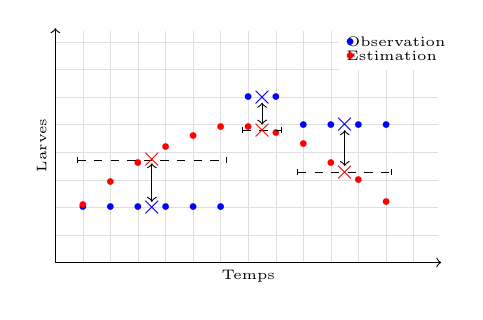
\begin{tikzpicture}[scale = 0.35]
 \draw [very thin, lightgray, opacity = 0.5] (0,0) grid (13.9, 8.4);
 \draw [->] (0, 0) -- (0, 8.5);
 \draw [->] (0, 0) -- (14, 0);
 \draw (1, 2) node{\tiny \textcolor{blue}{$\bullet$}};
 \draw (2, 2) node{\tiny \textcolor{blue}{$\bullet$}};
 \draw (3, 2) node{\tiny \textcolor{blue}{$\bullet$}};
 \draw (4, 2) node{\tiny \textcolor{blue}{$\bullet$}};
 \draw (5, 2) node{\tiny \textcolor{blue}{$\bullet$}};
 \draw (6, 2) node{\tiny \textcolor{blue}{$\bullet$}};
 \draw (7, 6) node{\tiny \textcolor{blue}{$\bullet$}};
 \draw (8, 6) node{\tiny \textcolor{blue}{$\bullet$}};
 \draw (9 , 5) node{\tiny \textcolor{blue}{$\bullet$}};
 \draw (10, 5) node{\tiny \textcolor{blue}{$\bullet$}};
 \draw (11, 5) node{\tiny \textcolor{blue}{$\bullet$}};
 \draw (12, 5) node{\tiny \textcolor{blue}{$\bullet$}};
 \draw (1, 2.1) node{\tiny\textcolor{red}{$\bullet$}};
 \draw (2, 2.9) node{\tiny\textcolor{red}{$\bullet$}};
 \draw (3, 3.6) node{\tiny\textcolor{red}{$\bullet$}};
 \draw (4, 4.2) node{\tiny\textcolor{red}{$\bullet$}};
 \draw (5, 4.6) node{\tiny\textcolor{red}{$\bullet$}};
 \draw (6, 4.9) node{\tiny\textcolor{red}{$\bullet$}};
 \draw (7, 4.9) node{\tiny\textcolor{red}{$\bullet$}};
 \draw (8, 4.7) node{\tiny\textcolor{red}{$\bullet$}};
 \draw (9, 4.3) node{\tiny\textcolor{red}{$\bullet$}};
 \draw (10, 3.6) node{\tiny\textcolor{red}{$\bullet$}};
 \draw (11, 3) node{\tiny\textcolor{red}{$\bullet$}};
 \draw (12, 2.2) node{\tiny\textcolor{red}{$\bullet$}};
 \draw [dashed] (0.8, 3.716) -- (6.2, 3.716) ;
 \draw [dashed] (6.8, 4.8) -- (8.2, 4.8) ;
 \draw [dashed] (8.8, 3.275) -- (12.2, 3.275) ;
 \draw (0.8, 3.616) -- (0.8, 3.816);
 \draw (6.2, 3.616) -- (6.2, 3.816);
 \draw (6.8, 4.7) -- (6.8, 4.9);
 \draw (8.2, 4.7) -- (8.2, 4.9);
 \draw (8.8, 3.175) -- (8.8, 3.375);
 \draw (12.2, 3.175) -- (12.2, 3.375);
 \draw (3.5, 3.716) node{\textcolor{red}{$\times$}};
 \draw (7.5, 4.8) node{\textcolor{red}{$\times$}}; 
 \draw (10.5, 3.275) node{\textcolor{red}{$\times$}};
 \draw (3.5, 2) node{\textcolor{blue}{$\times$}};
 \draw (7.5, 6) node{\textcolor{blue}{$\times$}}; 
 \draw (10.5, 5) node{\textcolor{blue}{$\times$}}; 
 \draw [<->] (3.5, 2.2) -- (3.5, 3.6);                  
 \draw [<->] (7.5, 5.8) -- (7.5, 5);
 \draw [<->] (10.5, 4.8) -- (10.5, 3.5);
 \draw [fill=white,white] (10.3, 7.01) rectangle (13.9, 8.4);
 \draw (12.35, 8) node {{\tiny Observation}};
 \draw (12.2, 7.5) node {{\tiny Estimation}};
 \draw (10.7, 8) node{\tiny\textcolor{blue}{$\bullet$}};
 \draw (10.7, 7.5) node{\tiny\textcolor{red}{$\bullet$}};
 \draw (6, 0.23) node[rotate = 180] {\textcolor{ForestGreen}{$\intercal$}};
 \draw (8, 0.23) node[rotate = 180] {\textcolor{ForestGreen}{$\intercal$}};
 \draw (12, 0.23) node[rotate = 180] {\textcolor{ForestGreen}{$\intercal$}};
 \draw (7, -0.5) node{\tiny \text{Temps}};
 \draw  (-0.5, 4.25) node{\rotatebox{90}{\tiny Larves}};
\end{tikzpicture}
\scriptsize
\caption[size = scriptsize]{\scriptsize Schéma illustrant le fonctionnement de la fonction objectif.}
\label{fig:calib}
\end{figure}
\end{multicols}
}
\only<2>{
 NB : On n'utilisera que le premier verger pour la calibration ; le second servira à la validation.
 }
\end{frame}










%% NSGA-II
\begin{frame}
 \frametitle{Algorithme d'optimisation}
 
 Algorithme choisi : \textbf{NSGA-II}
 
 \vspace{0.6cm} 
 
 \underline{Algorithme multicritères}
 \vspace{0.2cm}
 
 Nous avons trois critères
 \begin{itemize}
  \item  Sous-ensemble du front de Pareto
 \end{itemize}


 
 \vspace{0.6cm}
 \pause
 \underline{Algorithme génétique}
 \vspace{0.2cm}
 
 Les nouveaux jeux de paramètres sont obtenus par :
 \begin{itemize}
  \item croisement de solutions existantes
  \item mutation de certaines coordonnées
 \end{itemize}

 
\end{frame}






















%% CHOIX DES SOLUTIONS
\begin{frame}
 \frametitle{Choix des solutions}
 
 Il faut choisir une solution parmi un sous-ensemble du front de Pareto.
 
 \vspace{1cm}
 
 Regrouper les solutions semblables.
 
 \vspace{0.2cm}
 
 \textbf{Hypothèse : } Si deux jeux de paramètres sont proches, alors les solutions produites seront semblables.
 
 \vspace{0.2cm}
 
 \begin{itemize}
  \item  Effectuer une Classification Ascendante Hiérarchique sur les jeux de paramètres renvoyés par NSGA-II pour trouver différentes classes de solutions
  \item Explorer les classes de solutions pour identifier les solutions pertinentes
 \end{itemize}

%  
%  \vspace{0.2cm}
%  
%  $\longrightarrow$ Deux solutions sont semblables si les paramètres associées à chaque solution sont proches
%  
%  \vspace{0.2cm}
%  
%  $\longrightarrow$ Effectuer une Classification Ascendante Hiérarchique sur les jeux de paramètres renvoyés par NSGA-II pour trouver différentes classes de solutions
%  
%  \vspace{0.2cm}
%  
%  $\longrightarrow$ Explorer les classes de solutions pour identifier les solutions pertinentes
%  
\end{frame}












\begin{frame}
 \frametitle{Mise en œuvre}
 
 $\longrightarrow$ Modèle
 
 \vspace{0.6cm}
 
 $\longrightarrow$ Fonction de coût
 
 \vspace{0.6cm}
 
 $\longrightarrow$ Algorithme d'optimisation
 
 \vspace{0.6cm}
 
 $\longrightarrow$ Explorer les résultats
\end{frame}













%% SOLUTIONS 1
\begin{frame}
 \frametitle{Résultats}
\scriptsize
\begin{center}
\begin{tabular}{c}
  Solution 1 \\
  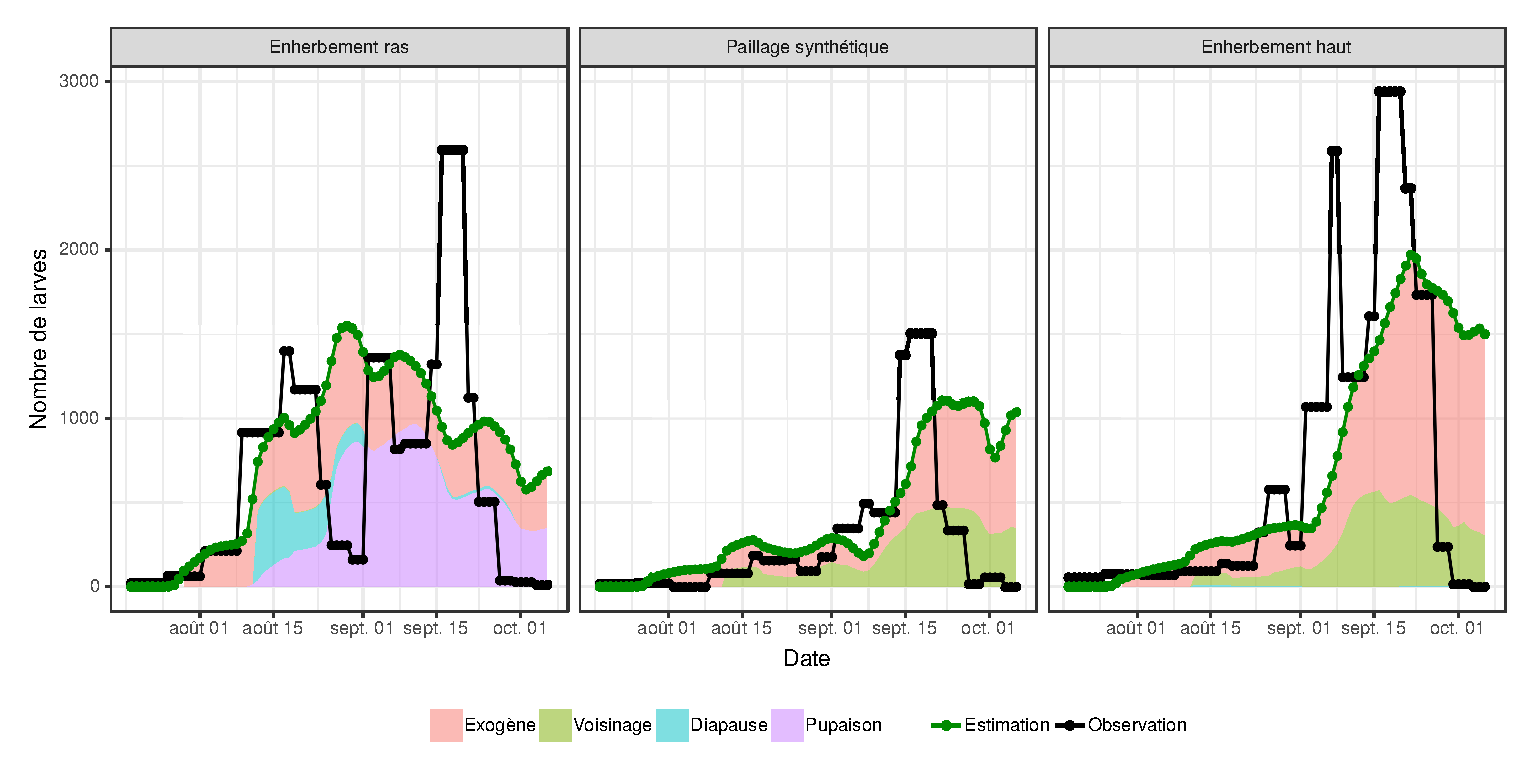
\epsfig{file = A1.eps, scale = 0.2}\\
  Solution 2\\
  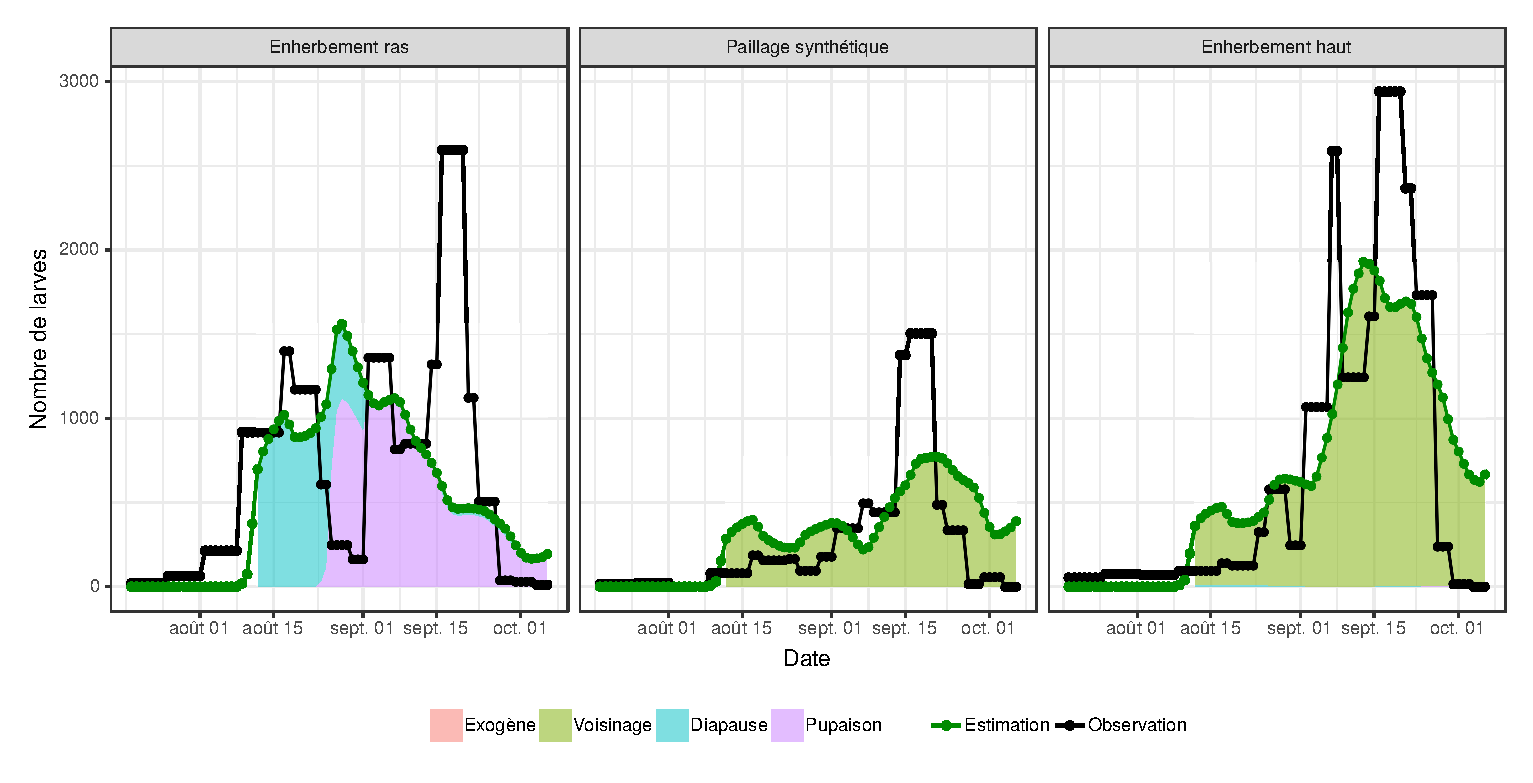
\epsfig{file = A2.eps, scale = 0.2} \\
  Solution 3\\
  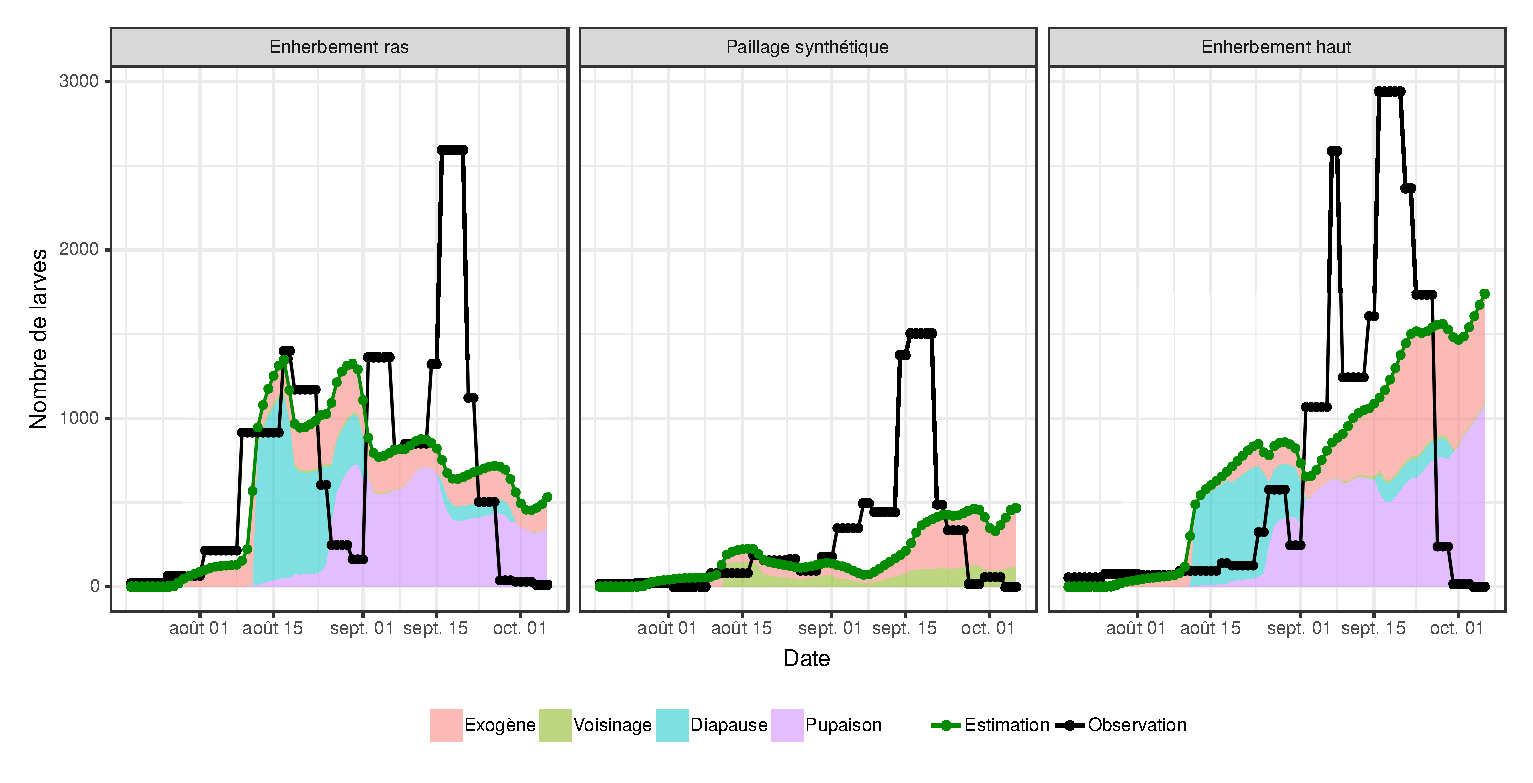
\epsfig{file = A3.eps, scale = 0.2}
\end{tabular}
\end{center}

%  \begin{multicols}{2}
%  Solution 1
% 
%  \vspace{3cm}
%  
%  Solution 2
% 
%  \vspace{3cm}
%  
%  Solution 3
%  
%  \vspace{15cm}
%  
%   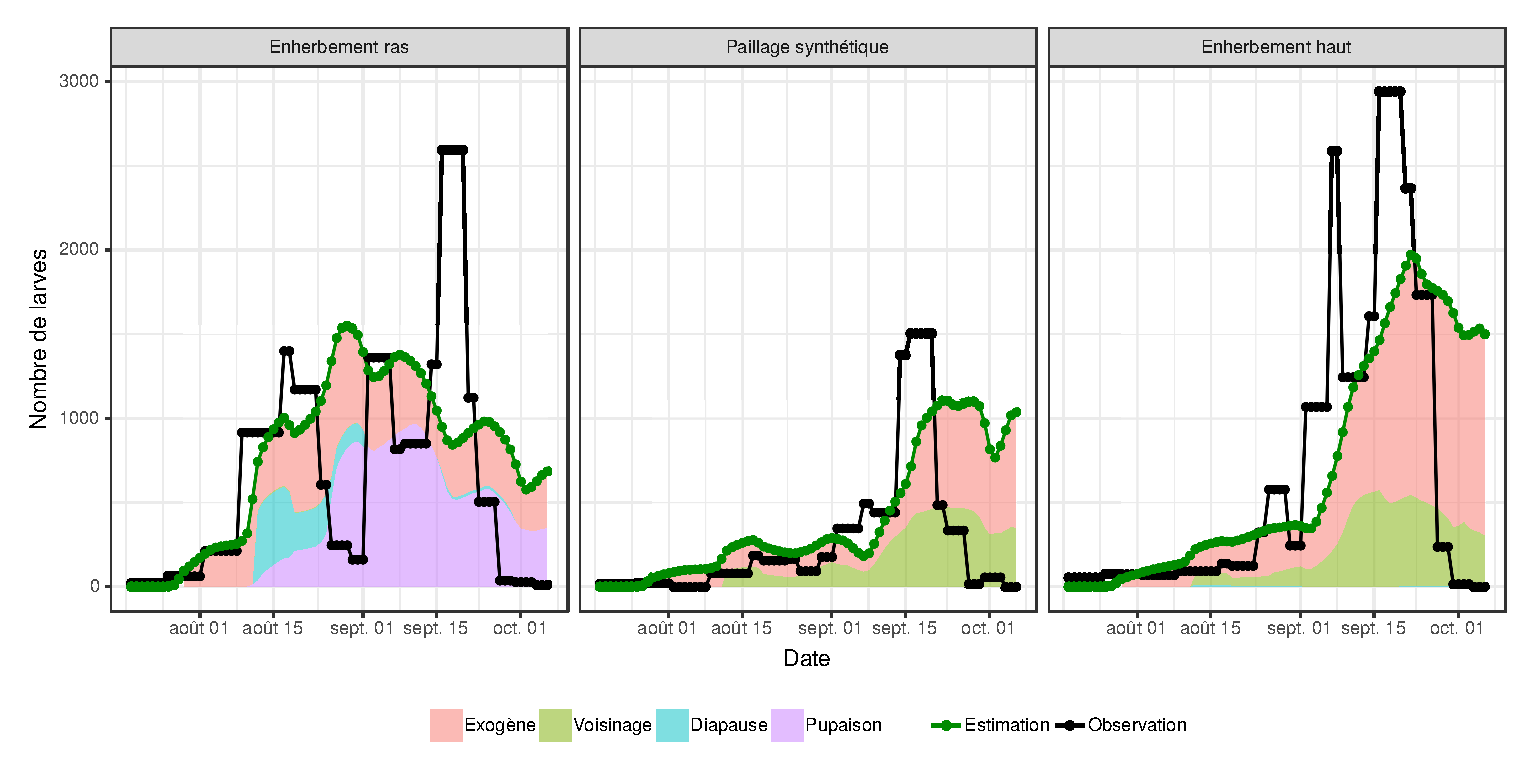
\epsfig{file = A1.eps, scale = 0.2}
%  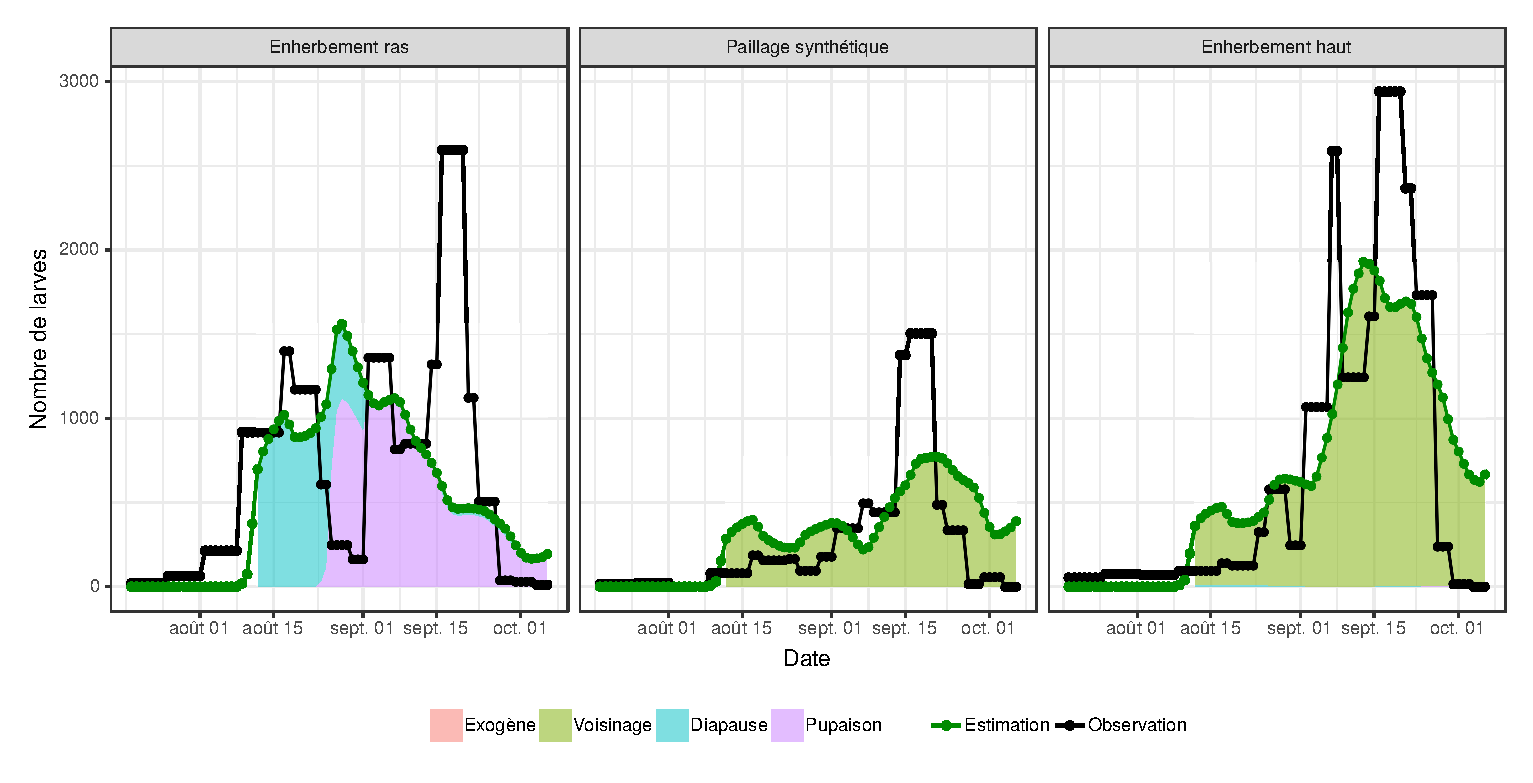
\epsfig{file = A2.eps, scale = 0.2}
%  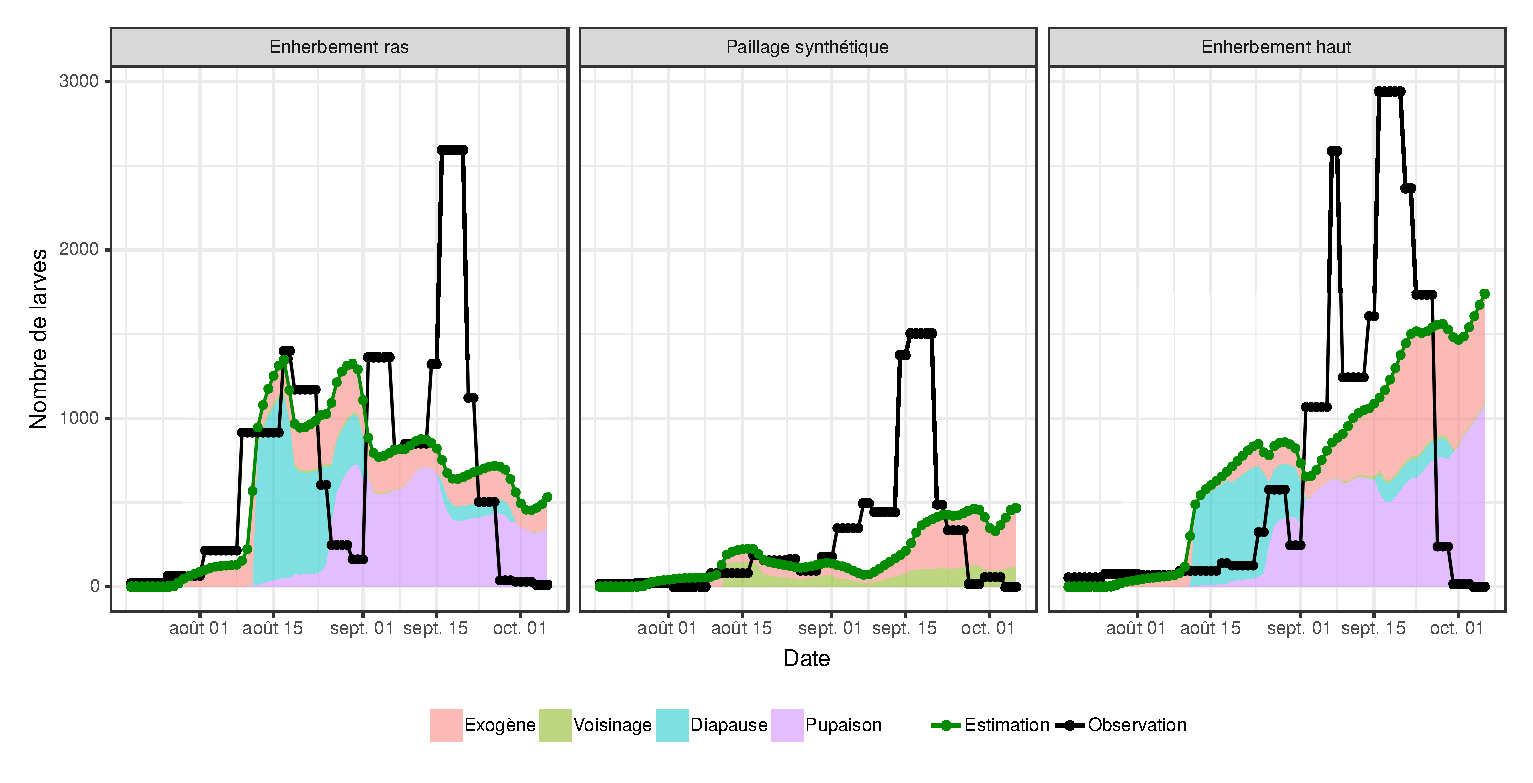
\epsfig{file = A3.eps, scale = 0.2}
% \end{multicols}

\end{frame}












%% SOLUTIONS 1
\begin{frame}
 \frametitle{Prise en compte de la température}
 
 
 \only<1>{
 \begin{center}
 \hspace{-2.3cm}
   \begin{tikzpicture}[transform canvas={scale=0.45}]
   \draw (-2,-5) node {\epsfig{file = pupaison.eps, scale = 0.6}};
\draw (0, 0) node{\small \textsc{sol}};
\draw [line width = 1.5mm, color = gray] (0.5, 0) -- (15, 0);
   
\draw (4.3,   4.5) rectangle (6, 5.5); % N
\draw (5.15,   5) node { $F_{i}$};
\draw (4.4, 5.7) node { $\textcolor{blue}{t}$};
% \pause

\draw (4.3,   7) rectangle (6,   8); % N exo
\draw (0.7,   4.5) rectangle (2.4,   5.5); % N voisins
\draw (8.4,   4.5) rectangle (10.1,  5.5); % N endo
\draw (5.15,   7.5) node { $F^\text{exo}_{i}$};
\draw (1.55,  5) node { $F^\text{endo}_{(j,k) \rightarrow i}$};
\draw (9.25,  5) node { $F^\text{endo}_{i\rightarrow i}$};
\draw (0.8, 5.7) node { $\textcolor{blue}{t}$};
\draw (4.4, 8.2) node { $\textcolor{blue}{t}$};
% \draw (8.5, 5.7) node { $\textcolor{blue}{t}$};
\draw [->,  line width=0.9] (5.15,   7 ) -- (5.15,  5.5);
\draw [->,  line width=0.9] (2.4,   5 ) -- (4.3,  5);
\draw [->,  line width=0.9] (8.4,   5) -- (6, 5);
%équations
\draw (11, 7.5) node {\scriptsize $F_{t, i} = F^\text{exo}_{t, i} + F^\text{endo}_{t, (j,k) \rightarrow i} + F^\text{endo}_{t, i\rightarrow i}$};
% \pause

\draw (4.3,   1.5) rectangle (6,   2.5); % L
\draw (5.15,   2) node { $L_{i}$};
\draw (4.8, 2.7) node { $\textcolor{blue}{t + d_{\ell}}$};
\draw (5.75, 4.1)     node { $R$};
\draw (5.8, 3.5)     node { $E_0$};
\draw (5.8, 2.9)     node { $\mu_\ell$};
\draw [->,  line width=0.9] (5.5,  4.5) -- (5.5, 2.5);
\draw [fill = white, white] (7.5, 6.8) rectangle (14.5, 8);
\draw (11, 7.5) node {\scriptsize $L_{t, i} = F_{t-d_\ell, i} \times R \times E_0 \times \mu_\ell$};
% \pause

% \draw (0.7,  -1.5) rectangle (2.4,  -2.5); %diap + mort
\draw (9.4,   1.5) rectangle (11.1,  2.5); % N pupe
% \draw (1.55, -2) node {\scriptsize Exclus};
\draw (10.25, 2) node { $F^{\text{pupe}}_{i}$};
\draw [line width=0.9]     (5.1,   1.5) -- (5.1,  -2);
% \draw [->,  line width=0.9] (5.1,  -2  ) -- (2.4,  -2);
\draw [line width=0.9] (5.1,  -2  ) -- (10.8,  -2);
\draw [->,  line width=0.9] (10.8,  -2 ) -- (10.8,  1.5);
\draw (10, 3.65) node { $\textcolor{blue}{t + d_{\ell} + d_{\text{p}}}$};
\draw (5.6, 0.4)   node { $\mu_{\text{sol}}^1$};
\draw (11.32, 0.4) node { $\mu_{\text{sol}}^2$};
\draw (7.9, -2.3)    node { \color{red} $p_{\text{p}}(t)$};
% \draw (3.8, -2.3)    node {\tiny $1-p_{\text{p}}$};
\draw (11.32, -0.42)  node { $\frac{1}{1 + \mathit{SR}}$};
\draw [fill = white, white] (7.5, 6.8) rectangle (14.5, 8);
\draw (11, 7.5) node {\scriptsize $F^{\text{pupe}}_{t,i} = L_{t-d_{\text{p}}, i} \times \mu_{\text{sol}}^1 \times p_{\text{p}} \times \frac{1}{1 + \mathit{SR}} \times \mu_{\text{sol}}^2$};
% % \pause

\draw (12.5, -1.5) rectangle (14.2, -2.5); %Diap
\draw (13.35,-2) node { $D_{i}$};
\draw (12.35, 2) node { $F^{\text{diap}}_{i}$};
\draw (11.5,  1.5) rectangle (13.2,  2.5); % N diap
\draw [line width=0.9]     (12.5, -2  ) -- (11.8, -2);
\draw [->,  line width=0.9] (11.8,  -2 ) -- (11.8,  1.5);
\draw [fill = white, white] (6.5, 6.8) rectangle (15.3, 8);
\draw (11, 7.5) node {\scriptsize $F^{\text{diap}}_{t,i} = D_{t, i} \times \frac{1}{1+\mathit{SR}} \times \mu_{\text{sol}}^2$};  
% \pause

\draw (9.1,   1.2) rectangle (13.5,  3.4); % N emer
\draw (11.3,  3) node { $F^{\text{endo}}_{i}$};
\draw [fill = white, white] (6.5, 6.8) rectangle (15.3, 8);
\draw (11, 7.5) node {\scriptsize $F^{\text{endo}}_{t,i} = F^{\text{diap}}_{t,i} + F^{\text{pupe}}_{t,i}$};
% \pause

 \draw (12.5,  4.5) rectangle (14.2,  5.5); % N degage

   % TEXTES CASES
\draw (13.35, 5) node { $F^\text{endo}_{i\rightarrow (j,k)}$};
% \draw (13, -1.3) node {\tiny $\textcolor{blue}{t + d_{\ell}}$};   
\draw (9.34, 5.65) node {  $\textcolor{blue}{t + d_{\ell} + d_{\text{p}}}$};
\draw (13.4, 5.75) node { $\textcolor{blue}{t + d_{\ell} + d_{\text{p}}}$};
\draw [line width=0.9]     (10.1, -2  ) -- (10.8, -2);
\draw [line width=0.9]     (11.3,  3.4) -- (11.3,  5);
\draw [->,  line width=0.9] (11.3,   5 ) -- (10.1,  5);
\draw [->,  line width=0.9] (11.3,   5 ) -- (12.5,  5);
\draw [->,  line width=0.9] (14.2,   5 ) -- (14.8,  5);
\draw [fill = white, white] (6.5, 6.8) rectangle (15.3, 8);
% \draw (11, 7.5) node {\scriptsize $F_{t, i \rightarrow j}^{\text{endo}} = \frac{I_{t, j} \times p_{\text{m}}^{\delta(i, j)}}{\sum_{n\in \{i,j,k\}} I_{t, n} \times p_{\text{m}}^{\delta(i, n)}}\times F_{t, i}^{\text{endo}}$};
\draw [fill = white, white] (6.05, 4) rectangle (8.35, 5.5);
\draw [->,  line width=0.9, dashed] (8.4,   5) -- (6, 5);
\draw [->, line width = 1.3, color = red] (4, -4) -- (7.4, -2.4);
\end{tikzpicture}
\end{center}
 }
 \only<2>{
\begin{center}
\begin{tabular}{cc}
 \scriptsize Sans température & \scriptsize Avec température \\
 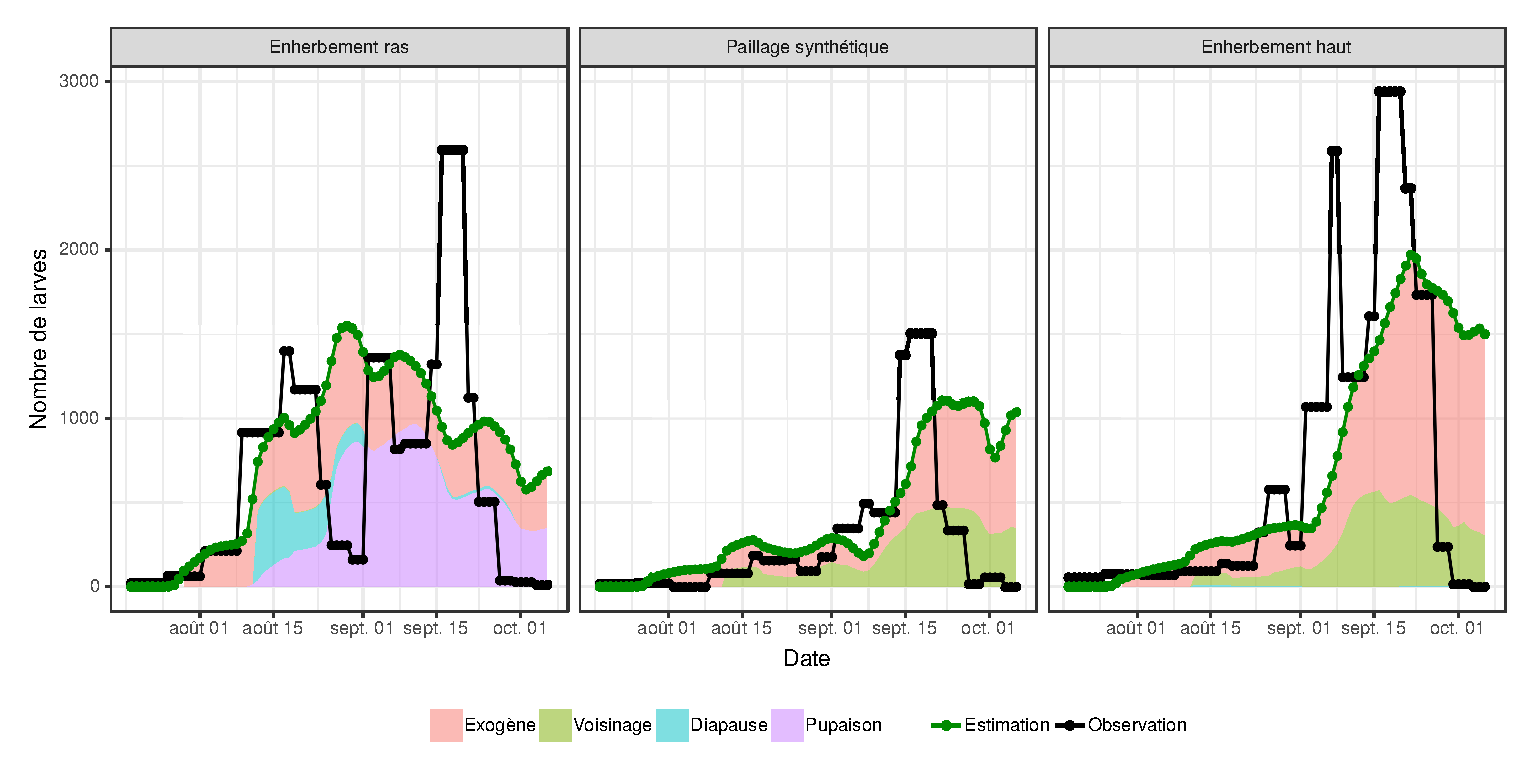
\epsfig{file = A1.eps, scale = 0.2} & 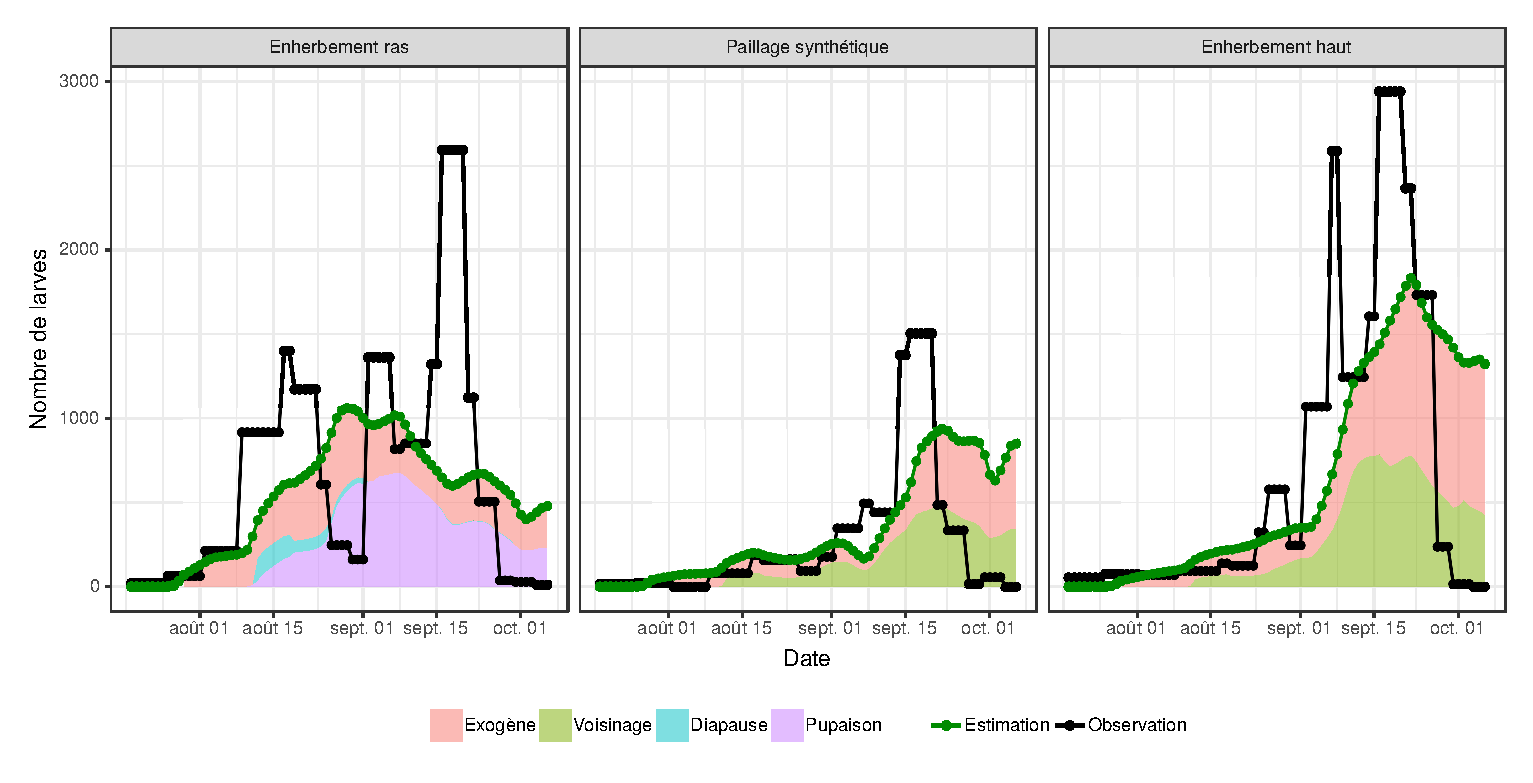
\epsfig{file = B1.eps, scale = 0.2}\\
 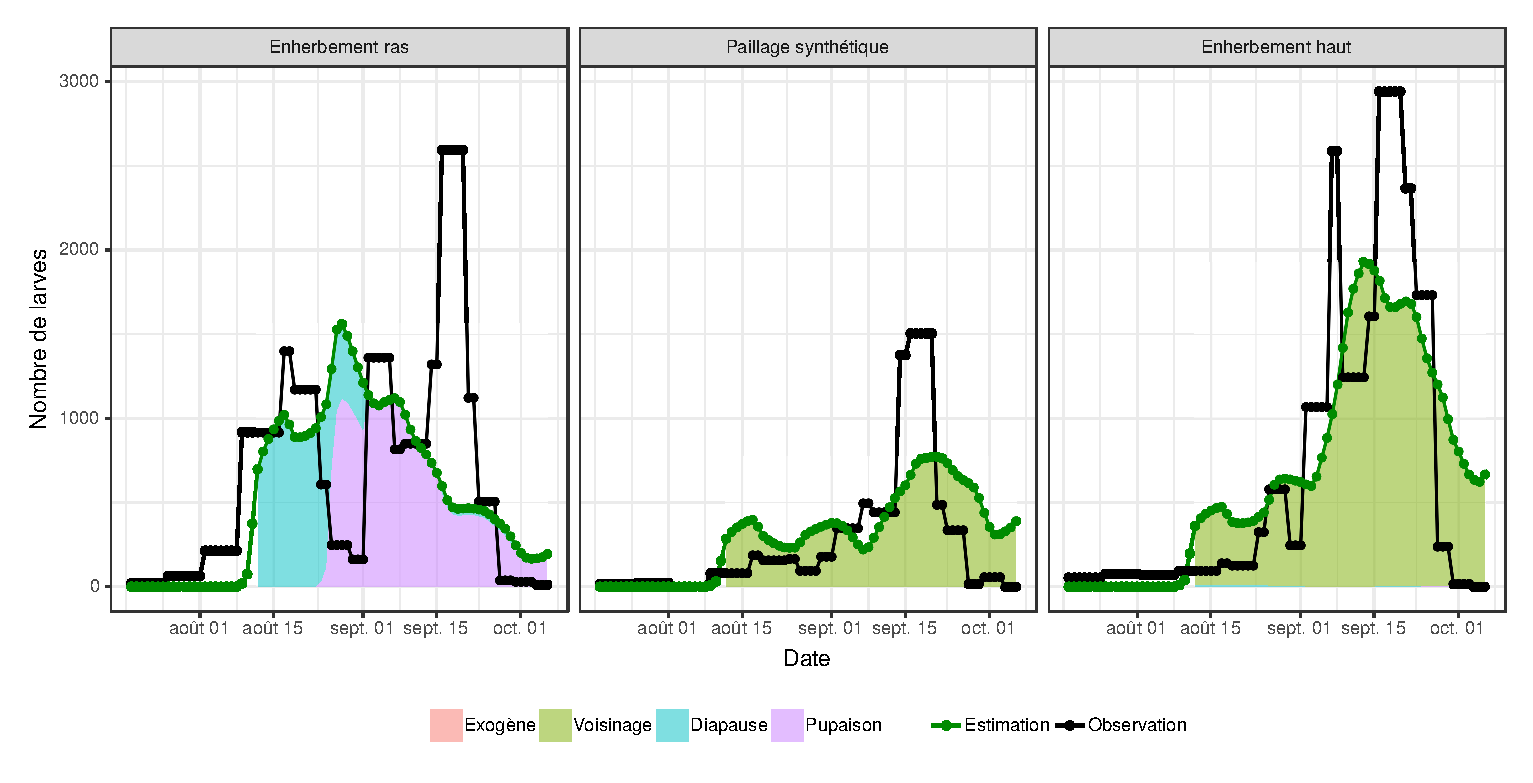
\epsfig{file = A2.eps, scale = 0.2} & 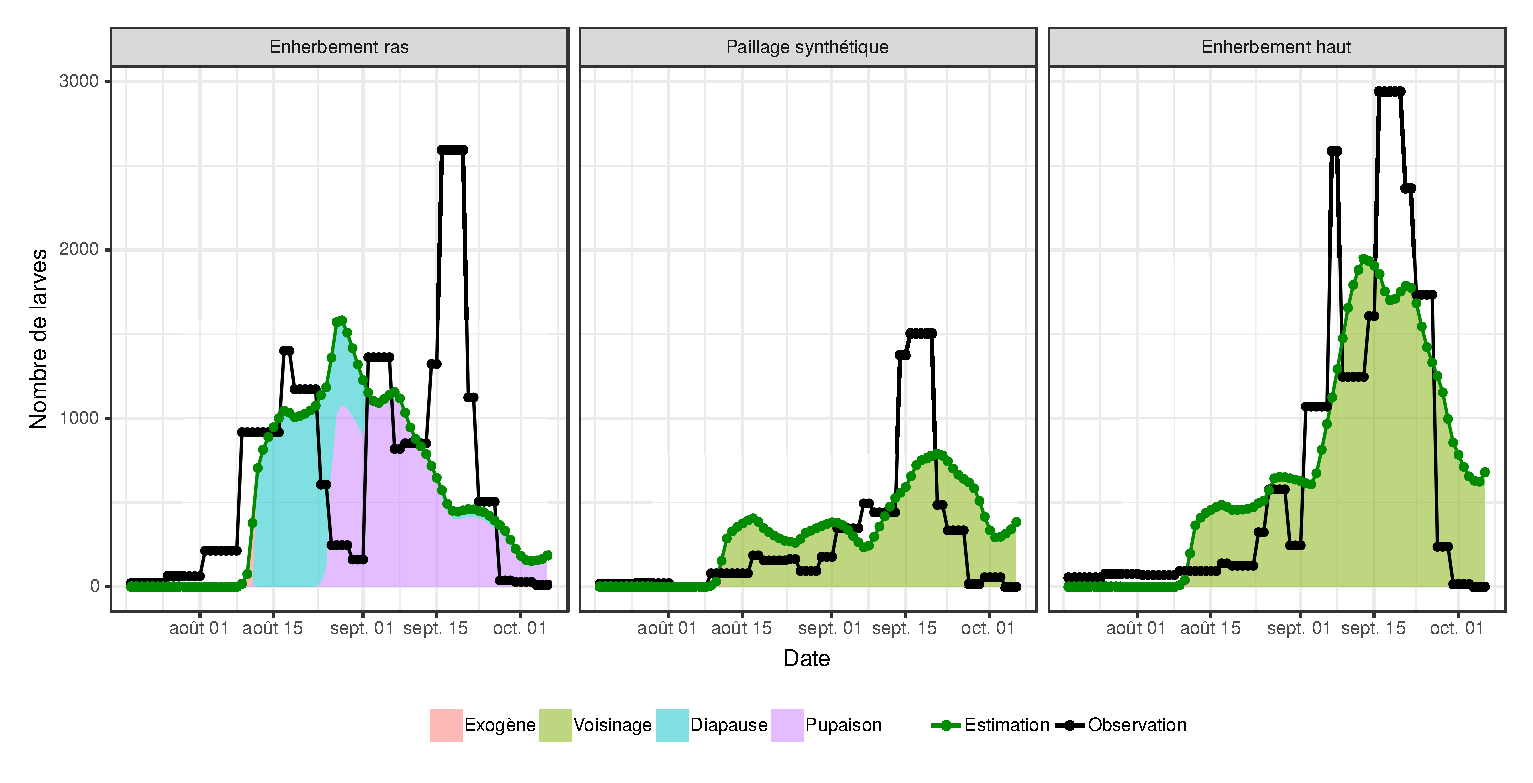
\epsfig{file = B2.eps, scale = 0.2} \\
 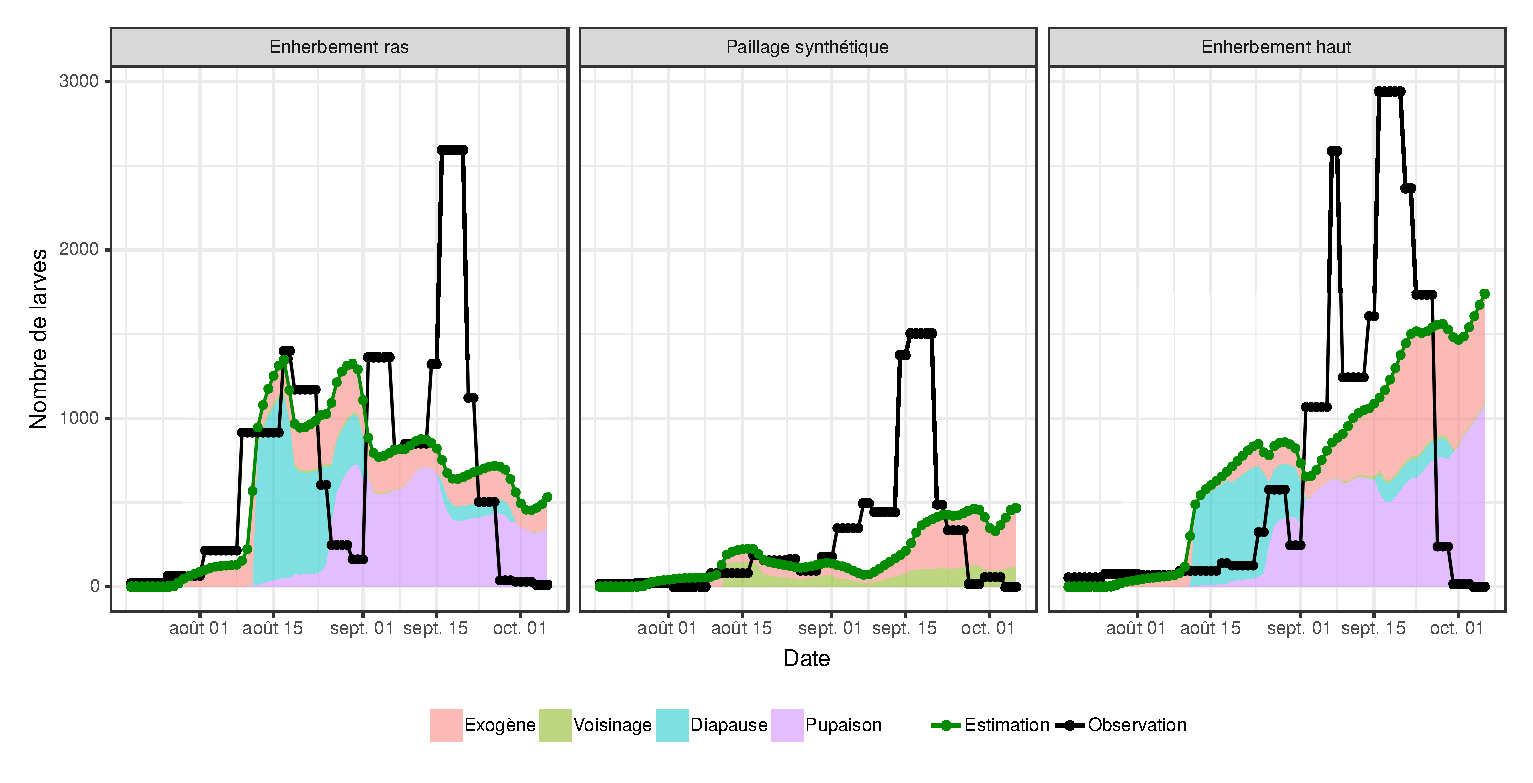
\epsfig{file = A3.eps, scale = 0.2} & 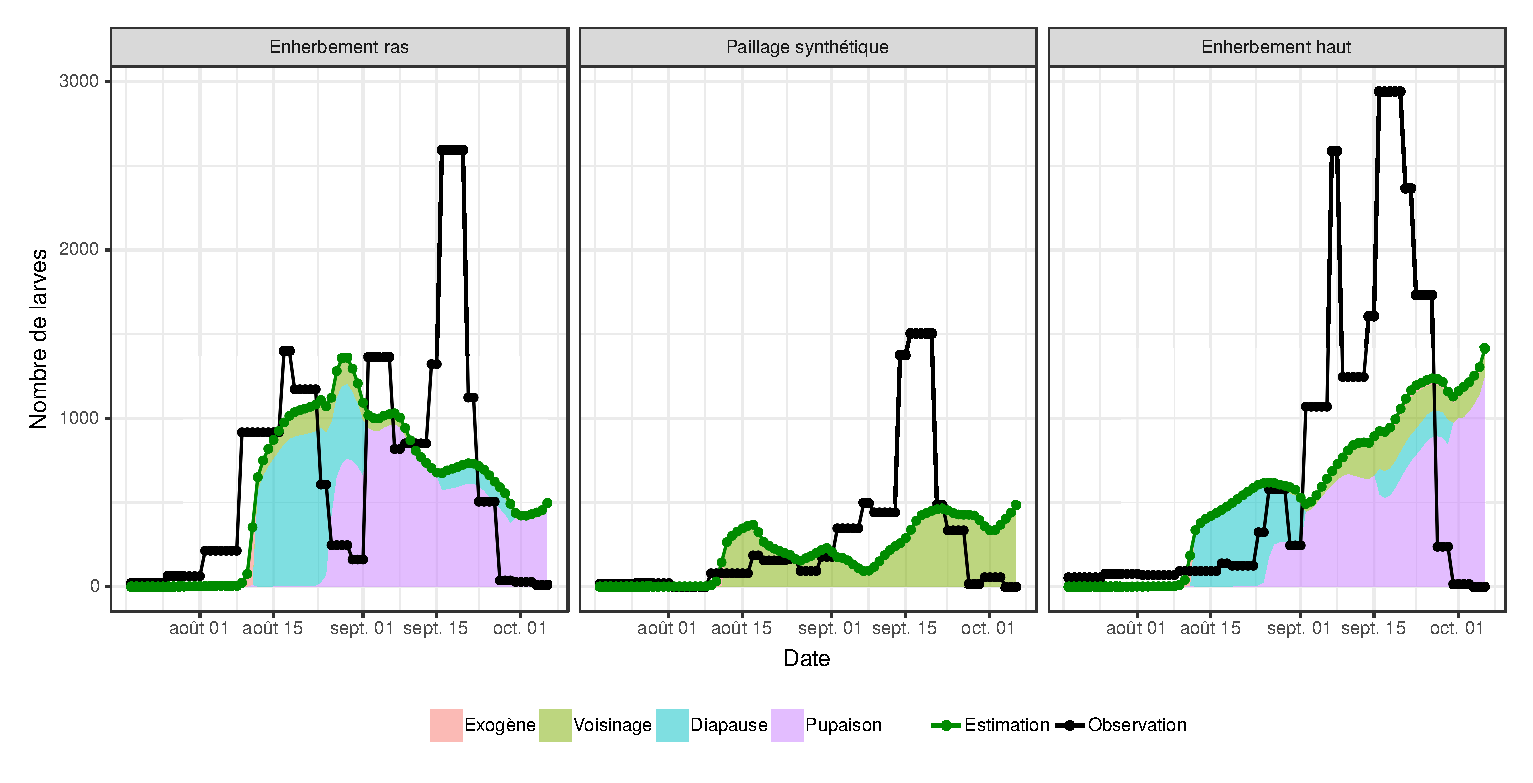
\epsfig{file = B3.eps, scale = 0.2}
\end{tabular}
\end{center}
 }
 

 
\end{frame}



















%% SOLUTIONS 1
\begin{frame}
 \frametitle{Stade phénologique des inflorescences}
 
\only<1>{
\begin{center}
\vspace{0.5cm}
\hspace{-2cm}
   \begin{tikzpicture}[transform canvas={scale=0.45}]
\draw (-3, -5) node {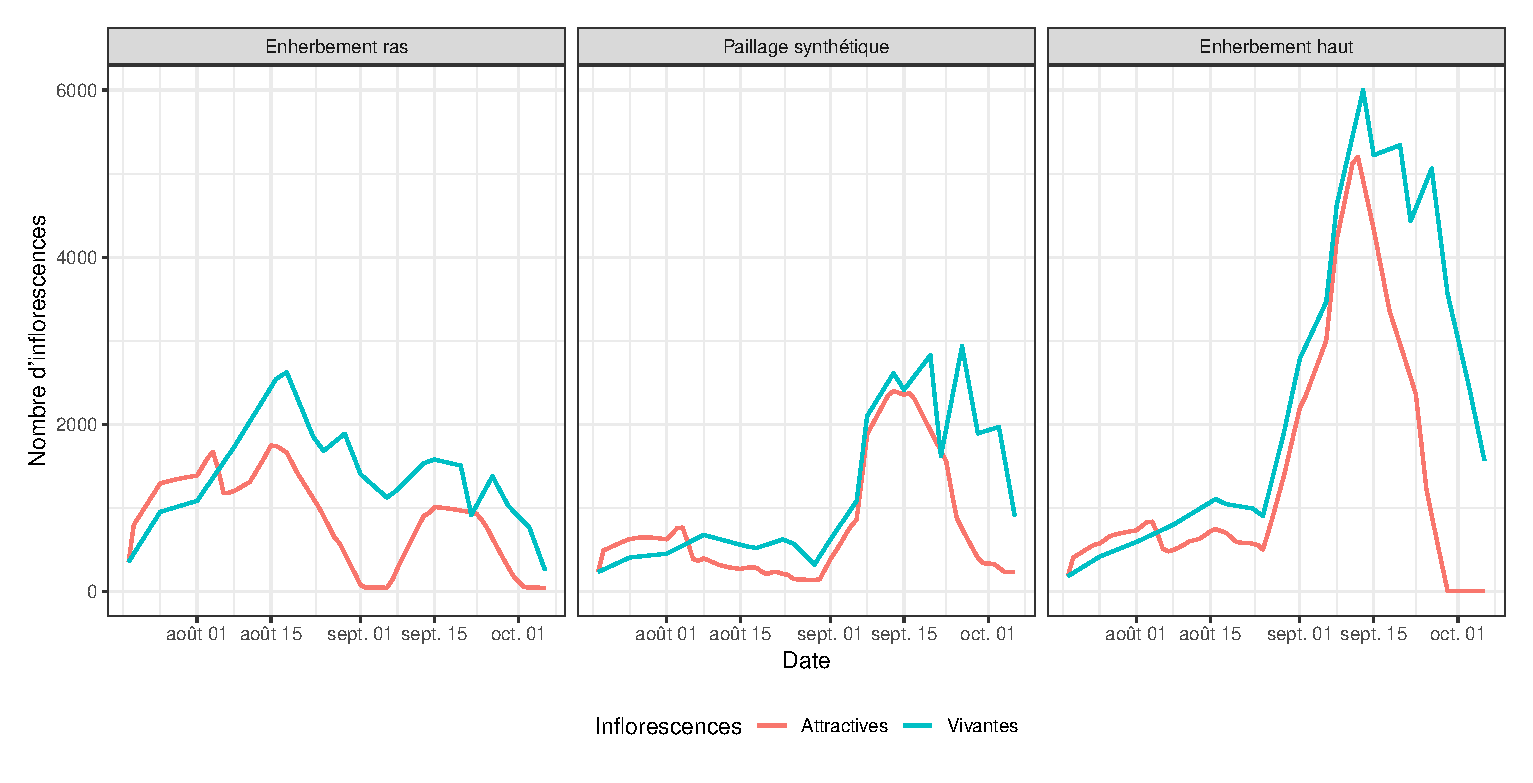
\epsfig{file = inflos_CDE.eps, scale = 0.6}};
   \draw (0, 0) node{\small \textsc{sol}};
\draw [line width = 1.5mm, color = gray] (0.5, 0) -- (15, 0);
   
\draw (4.3,   4.5) rectangle (6, 5.5); % N
\draw (5.15,   5) node { $F_{i}$};
\draw (4.4, 5.7) node { $\textcolor{blue}{t}$};
% \pause

\draw [red] (4.3,   7) rectangle (6,   8); % N exo
\draw (0.7,   4.5) rectangle (2.4,   5.5); % N voisins
\draw (8.4,   4.5) rectangle (10.1,  5.5); % N endo
\draw (5.15,   7.5) node {\color{red} $F^\text{exo}_{i}$};
\draw (1.55,  5) node { $F^\text{endo}_{(j,k) \rightarrow i}$};
\draw (9.25,  5) node { $F^\text{endo}_{i\rightarrow i}$};
\draw (0.8, 5.7) node { $\textcolor{blue}{t}$};
\draw (4.4, 8.2) node { $\textcolor{blue}{t}$};
% \draw (8.5, 5.7) node { $\textcolor{blue}{t}$};
\draw [->,  line width=0.9] (5.15,   7 ) -- (5.15,  5.5);
\draw [->,  line width=0.9] (2.4,   5 ) -- (4.3,  5);
\draw [->,  line width=0.9] (8.4,   5) -- (6, 5);
%équations
\draw (11, 7.5) node {\scriptsize $F_{t, i} = F^\text{exo}_{t, i} + F^\text{endo}_{t, (j,k) \rightarrow i} + F^\text{endo}_{t, i\rightarrow i}$};
% \pause

\draw (4.3,   1.5) rectangle (6,   2.5); % L
\draw (5.15,   2) node { $L_{i}$};
\draw (4.8, 2.7) node { $\textcolor{blue}{t + d_{\ell}}$};
\draw (5.75, 4.1)     node {\color{red} $R$};
\draw (5.8, 3.5)     node { $E_0$};
\draw (5.8, 2.9)     node { $\mu_\ell$};
\draw [->,  line width=0.9] (5.5,  4.5) -- (5.5, 2.5);
\draw [fill = white, white] (7.5, 6.8) rectangle (14.5, 8);
\draw (11, 7.5) node {\scriptsize $L_{t, i} = F_{t-d_\ell, i} \times R \times E_0 \times \mu_\ell$};
% \pause

% \draw (0.7,  -1.5) rectangle (2.4,  -2.5); %diap + mort
\draw (9.4,   1.5) rectangle (11.1,  2.5); % N pupe
% \draw (1.55, -2) node {\scriptsize Exclus};
\draw (10.25, 2) node { $F^{\text{pupe}}_{i}$};
\draw [line width=0.9]     (5.1,   1.5) -- (5.1,  -2);
% \draw [->,  line width=0.9] (5.1,  -2  ) -- (2.4,  -2);
\draw [line width=0.9] (5.1,  -2  ) -- (10.8,  -2);
\draw [->,  line width=0.9] (10.8,  -2 ) -- (10.8,  1.5);
\draw (10, 3.65) node { $\textcolor{blue}{t + d_{\ell} + d_{\text{p}}}$};
\draw (5.6, 0.4)   node { $\mu_{\text{sol}}^1$};
\draw (11.32, 0.4) node { $\mu_{\text{sol}}^2$};
\draw (7.9, -2.3)    node { $p_{\text{p}}$};
% \draw (3.8, -2.3)    node {\tiny $1-p_{\text{p}}$};
\draw (11.32, -0.42)  node { $\frac{1}{1 + \mathit{SR}}$};
\draw [fill = white, white] (7.5, 6.8) rectangle (14.5, 8);
\draw (11, 7.5) node {\scriptsize $F^{\text{pupe}}_{t,i} = L_{t-d_{\text{p}}, i} \times \mu_{\text{sol}}^1 \times p_{\text{p}} \times \frac{1}{1 + \mathit{SR}} \times \mu_{\text{sol}}^2$};
% % \pause

\draw (12.5, -1.5) rectangle (14.2, -2.5); %Diap
\draw (13.35,-2) node { $D_{i}$};
\draw (12.35, 2) node { $F^{\text{diap}}_{i}$};
\draw (11.5,  1.5) rectangle (13.2,  2.5); % N diap
\draw [line width=0.9]     (12.5, -2  ) -- (11.8, -2);
\draw [->,  line width=0.9] (11.8,  -2 ) -- (11.8,  1.5);
\draw [fill = white, white] (6.5, 6.8) rectangle (15.3, 8);
\draw (11, 7.5) node {\scriptsize $F^{\text{diap}}_{t,i} = D_{t, i} \times \frac{1}{1+\mathit{SR}} \times \mu_{\text{sol}}^2$};  
% \pause

\draw (9.1,   1.2) rectangle (13.5,  3.4); % N emer
\draw (11.3,  3) node { $F^{\text{endo}}_{i}$};
\draw [fill = white, white] (6.5, 6.8) rectangle (15.3, 8);
\draw (11, 7.5) node {\scriptsize $F^{\text{endo}}_{t,i} = F^{\text{diap}}_{t,i} + F^{\text{pupe}}_{t,i}$};
% \pause

 \draw (12.5,  4.5) rectangle (14.2,  5.5); % N degage

   % TEXTES CASES
\draw (13.35, 5) node { $F^\text{endo}_{i\rightarrow (j,k)}$};
% \draw (13, -1.3) node {\tiny $\textcolor{blue}{t + d_{\ell}}$};   
\draw (9.34, 5.65) node {  $\textcolor{blue}{t + d_{\ell} + d_{\text{p}}}$};
\draw (13.4, 5.75) node { $\textcolor{blue}{t + d_{\ell} + d_{\text{p}}}$};
\draw [line width=0.9]     (10.1, -2  ) -- (10.8, -2);
\draw [line width=0.9]     (11.3,  3.4) -- (11.3,  5);
\draw [->,  line width=0.9] (11.3,   5 ) -- (10.1,  5);
\draw [->,  line width=0.9] (11.3,   5 ) -- (12.5,  5);
\draw [->,  line width=0.9] (14.2,   5 ) -- (14.8,  5);
\draw [fill = white, white] (6.5, 6.8) rectangle (15.3, 8);
\draw [->, line width = 1.3, color = red] (9, 7.5) -- (6, 7.5);
\draw [->, line width = 1.3, color = red] (0, -1) -- (5.6, 4.1);
\draw [line width = 1.3, color = red] (11.3, 4.5) circle (1.5);
\draw [fill = white, white] (6.05, 4) rectangle (8.35, 5.5);
\draw [->,  line width=0.9, dashed] (8.4,   5) -- (6, 5);
% \draw (11, 7.5) node {\scriptsize $F_{t, i \rightarrow j}^{\text{endo}} = \frac{I_{t, j} \times p_{\text{m}}^{\delta(i, j)}}{\sum_{n\in \{i,j,k\}} I_{t, n} \times p_{\text{m}}^{\delta(i, n)}}\times F_{t, i}^{\text{endo}}$};
% \draw [->, line width = 1.3, color = red] (0, 2) -- (7.4, -2.2);
\end{tikzpicture}
\end{center}
}
\only<2>{
%  \begin{figure}
%   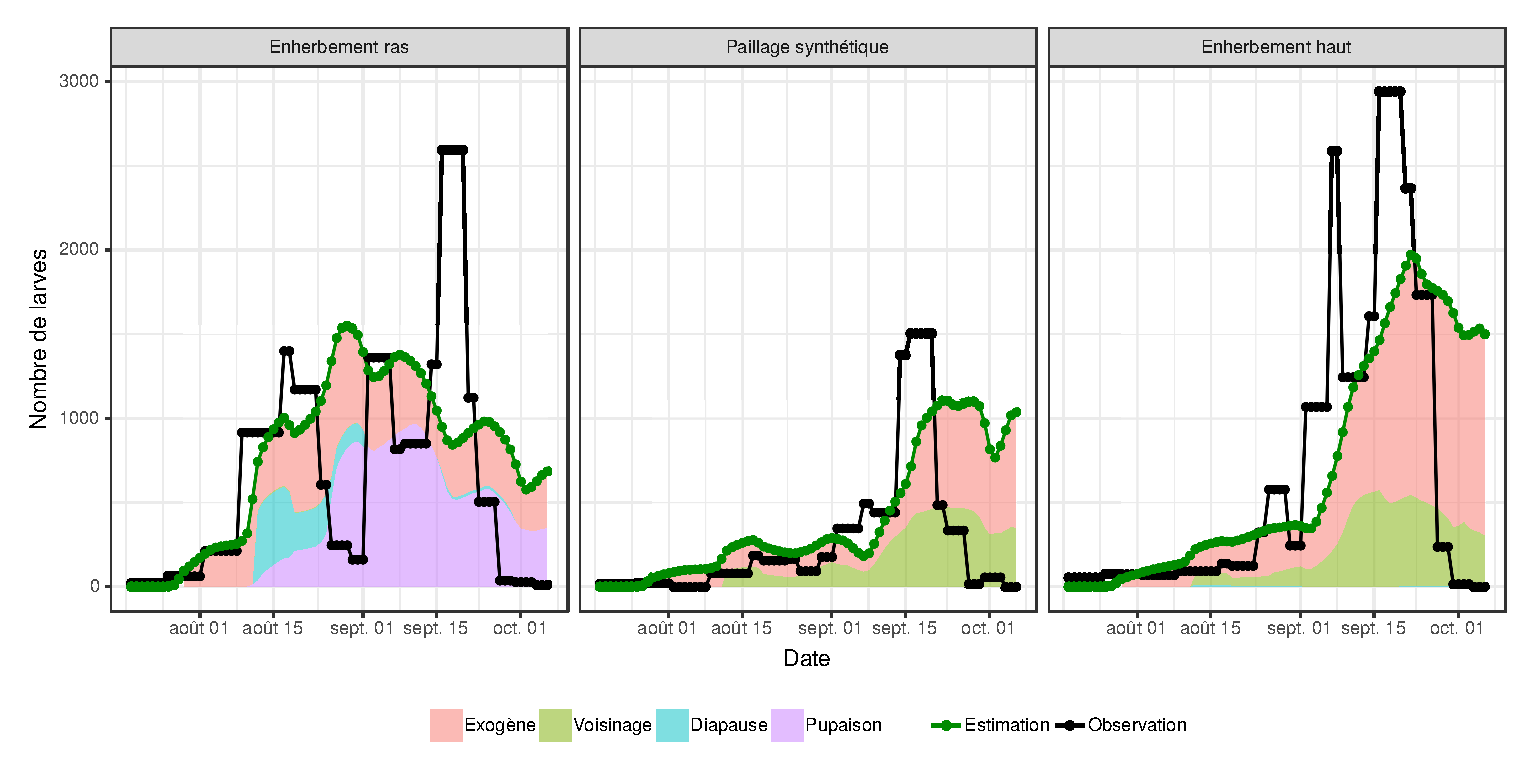
\epsfig{file = A1.eps, scale = 0.2}
%   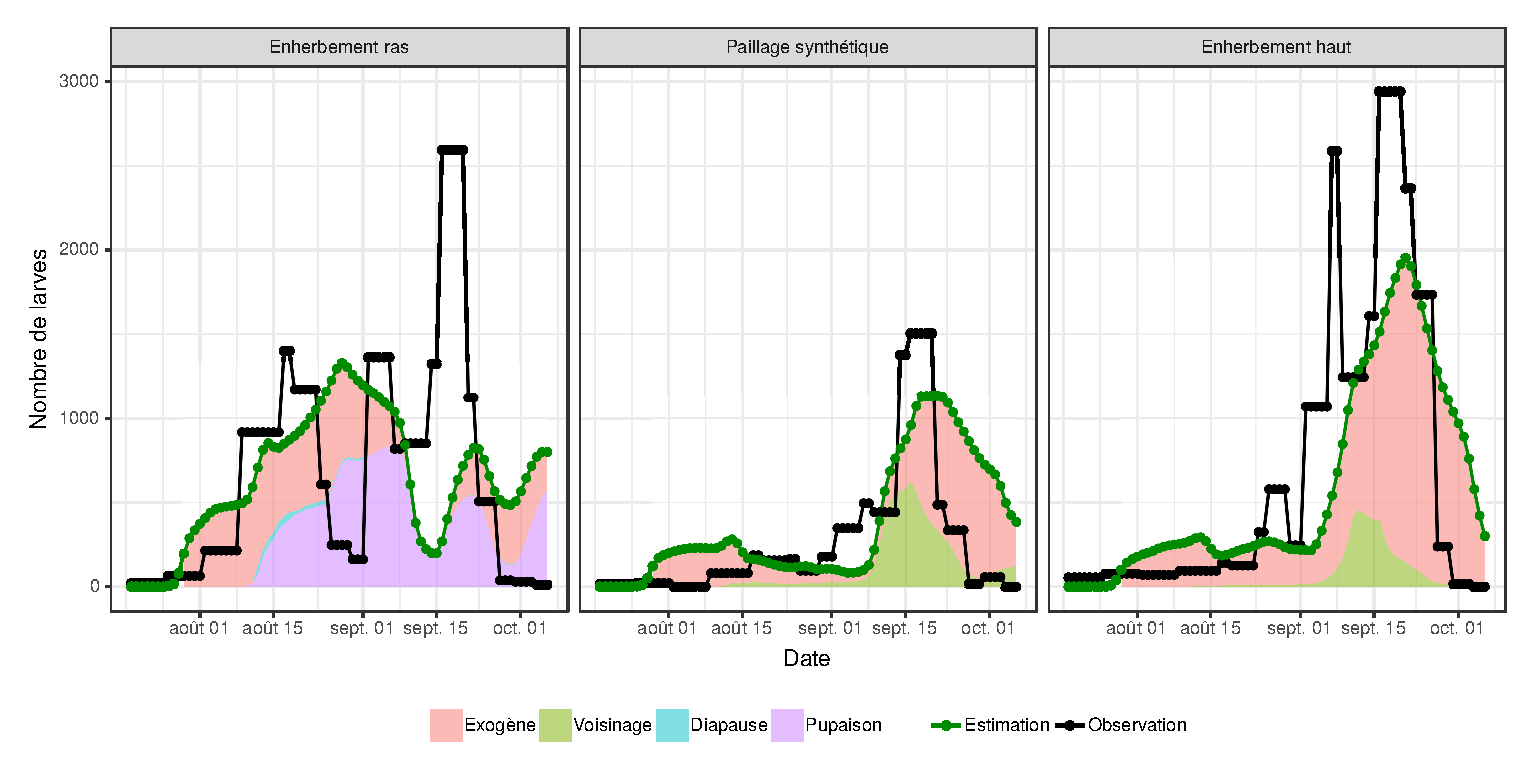
\epsfig{file = C1.eps, scale = 0.2}
%   
%   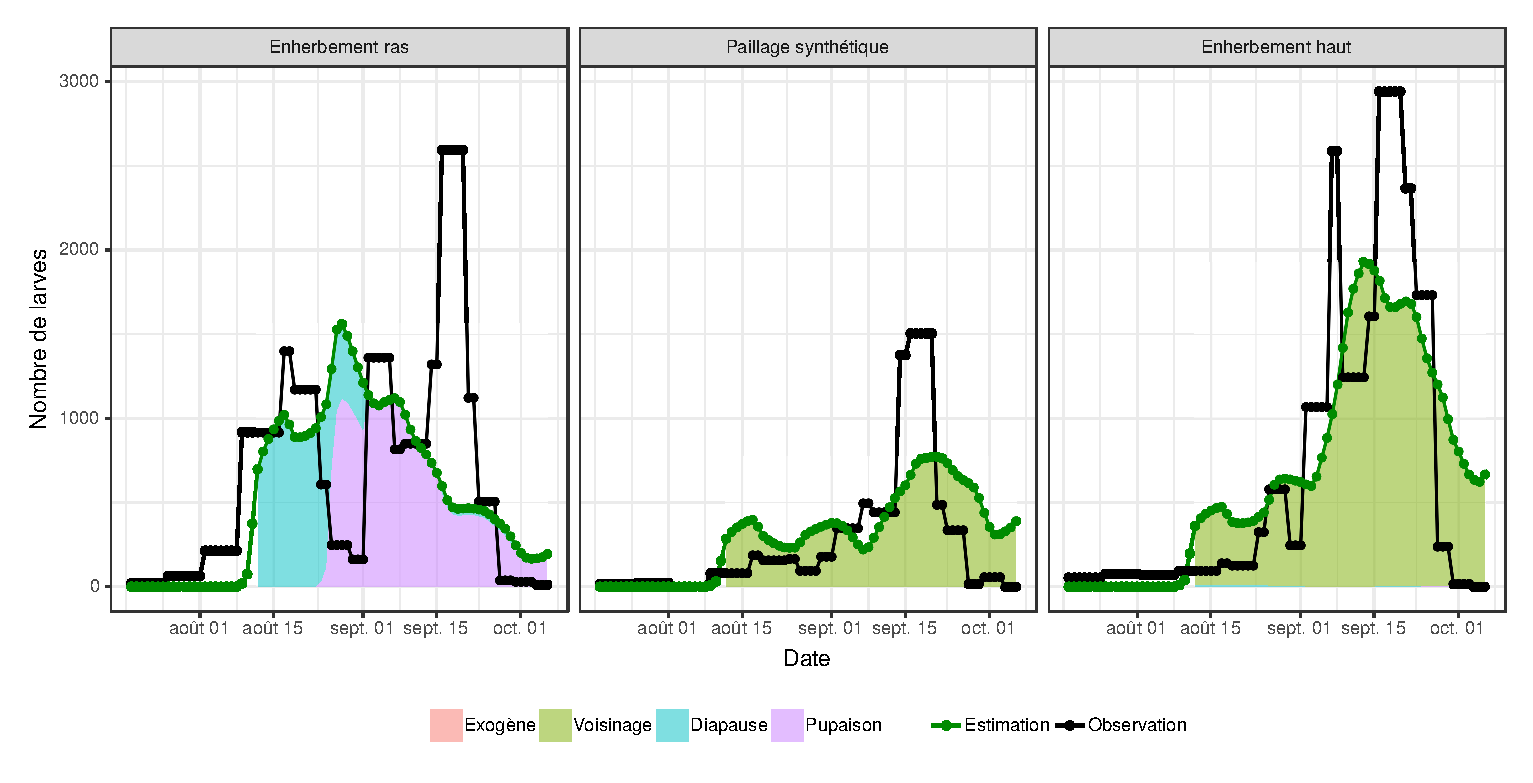
\epsfig{file = A2.eps, scale = 0.2}
%   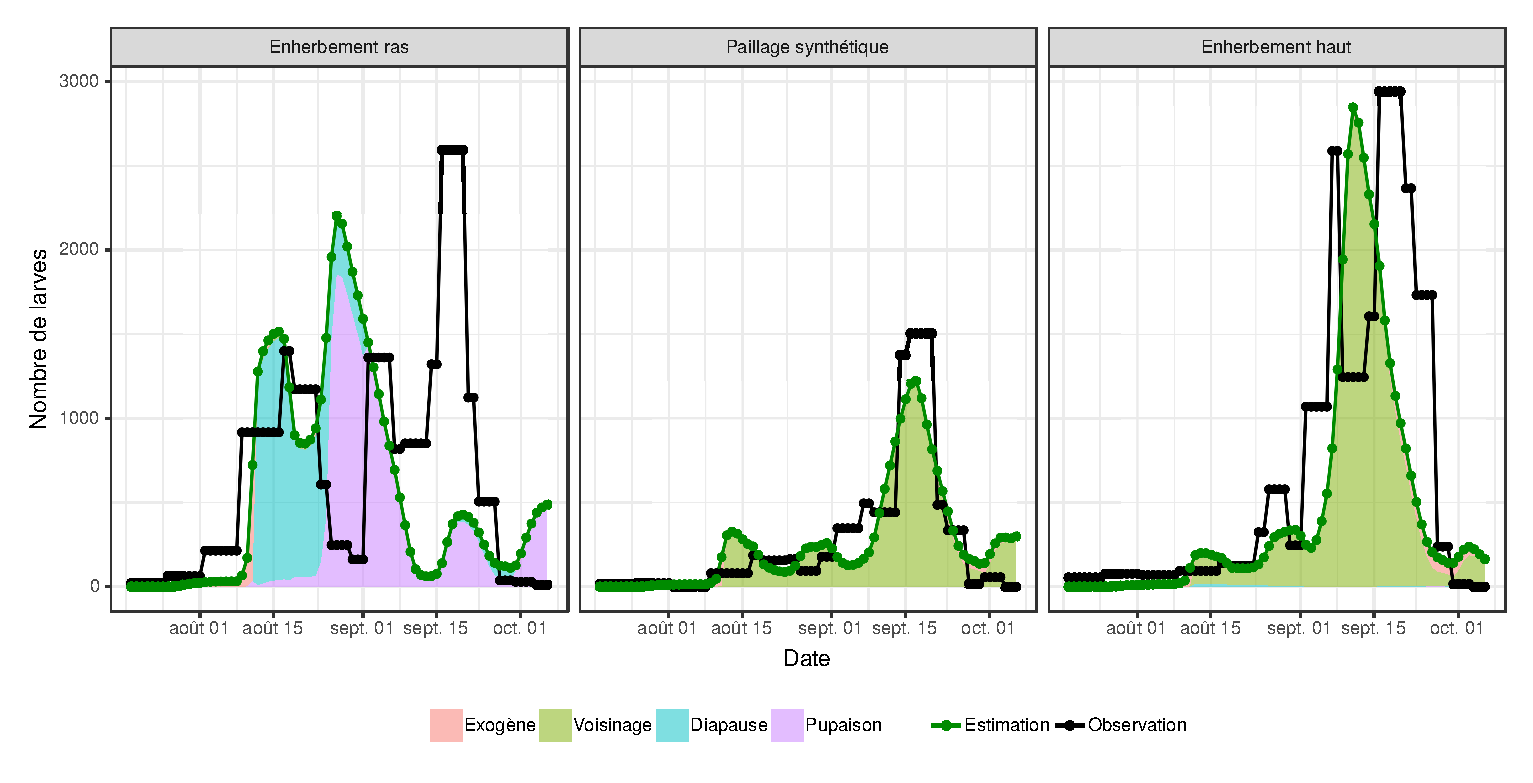
\epsfig{file = C2.eps, scale = 0.2}
%   
%   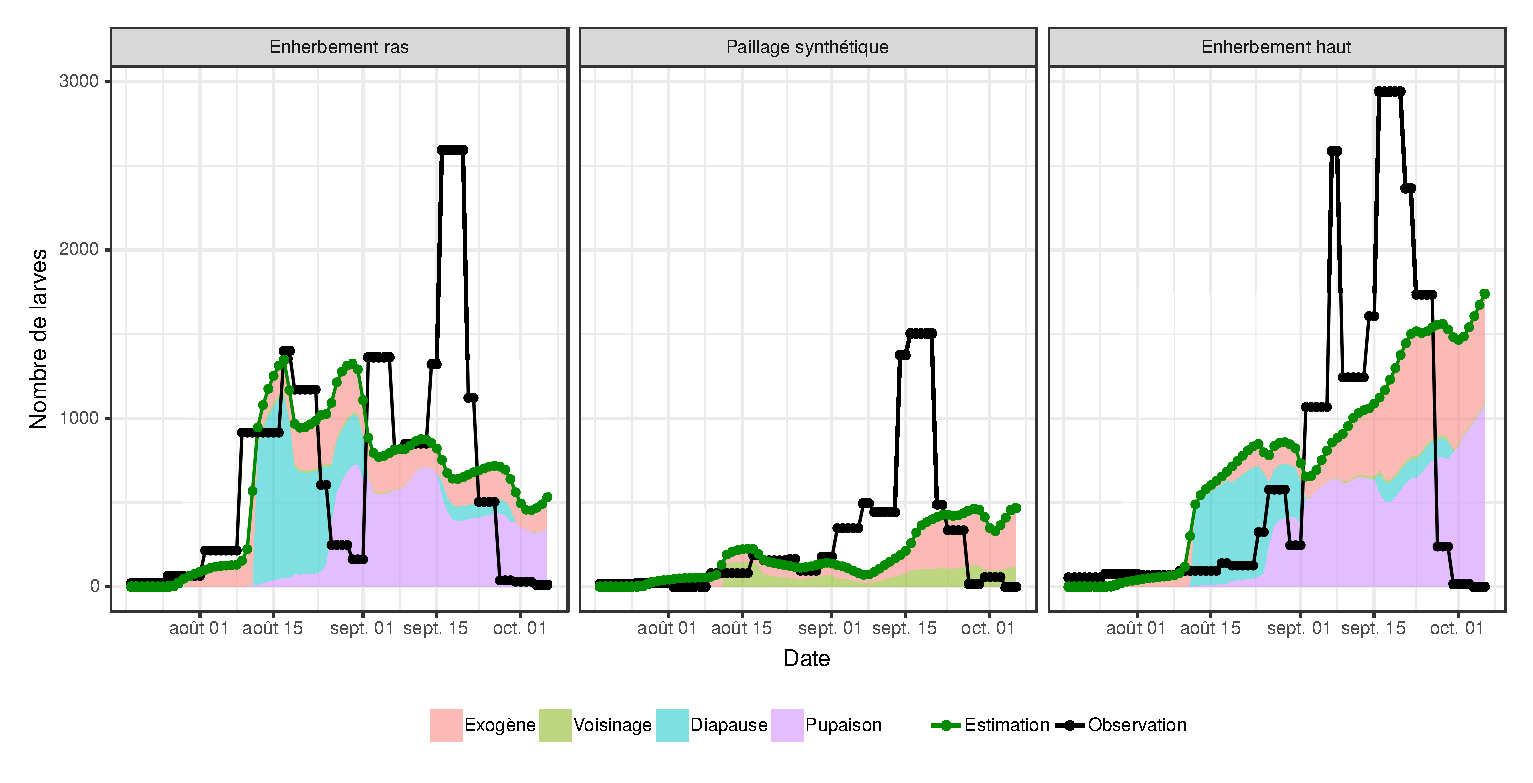
\epsfig{file = A3.eps, scale = 0.2}
%   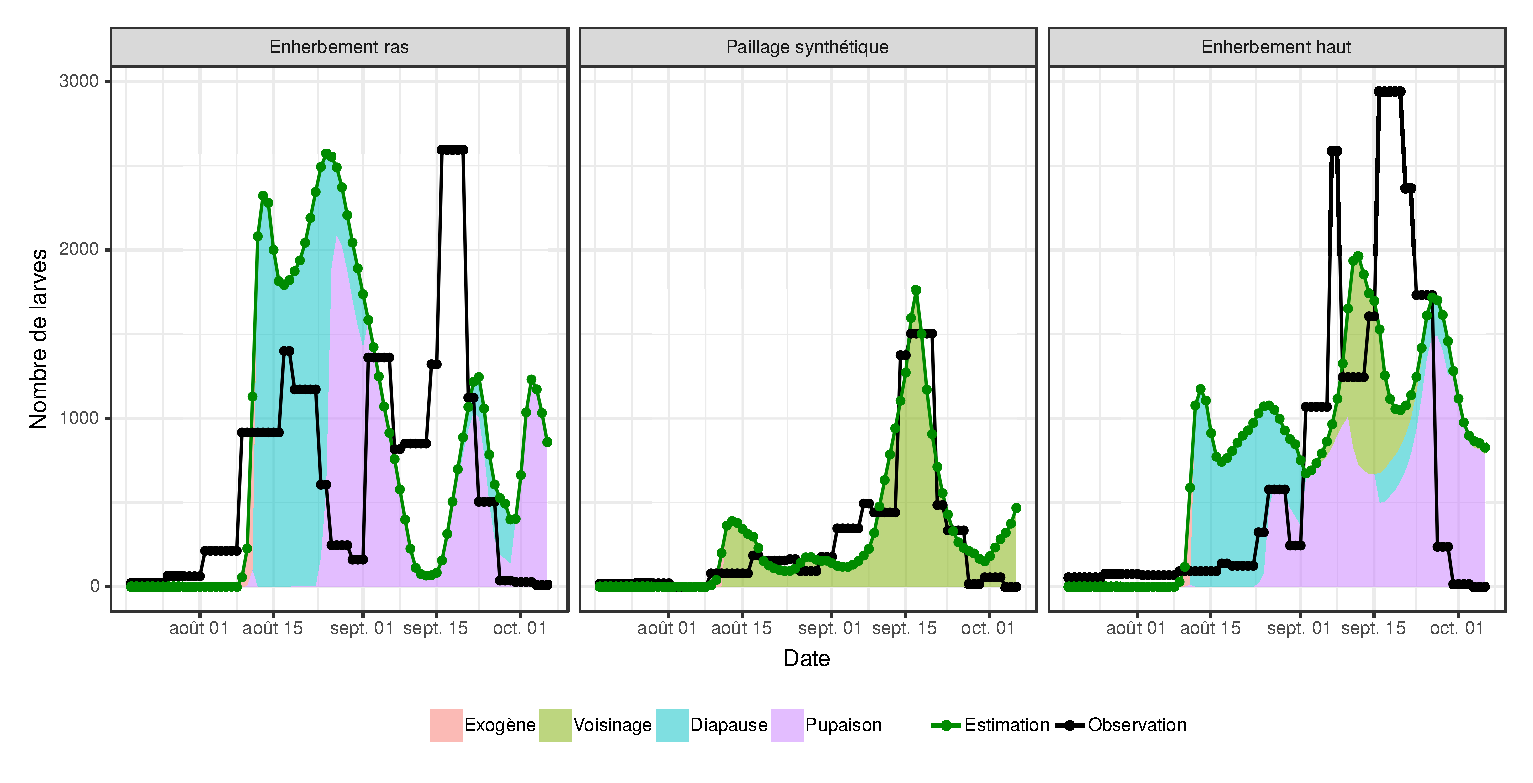
\epsfig{file = C3.eps, scale = 0.2} 
%   \end{figure}
\begin{center}
\begin{tabular}{cc}
 \scriptsize Inflorescences vivantes & \scriptsize Inflorescences aux stades C, D et E \\
 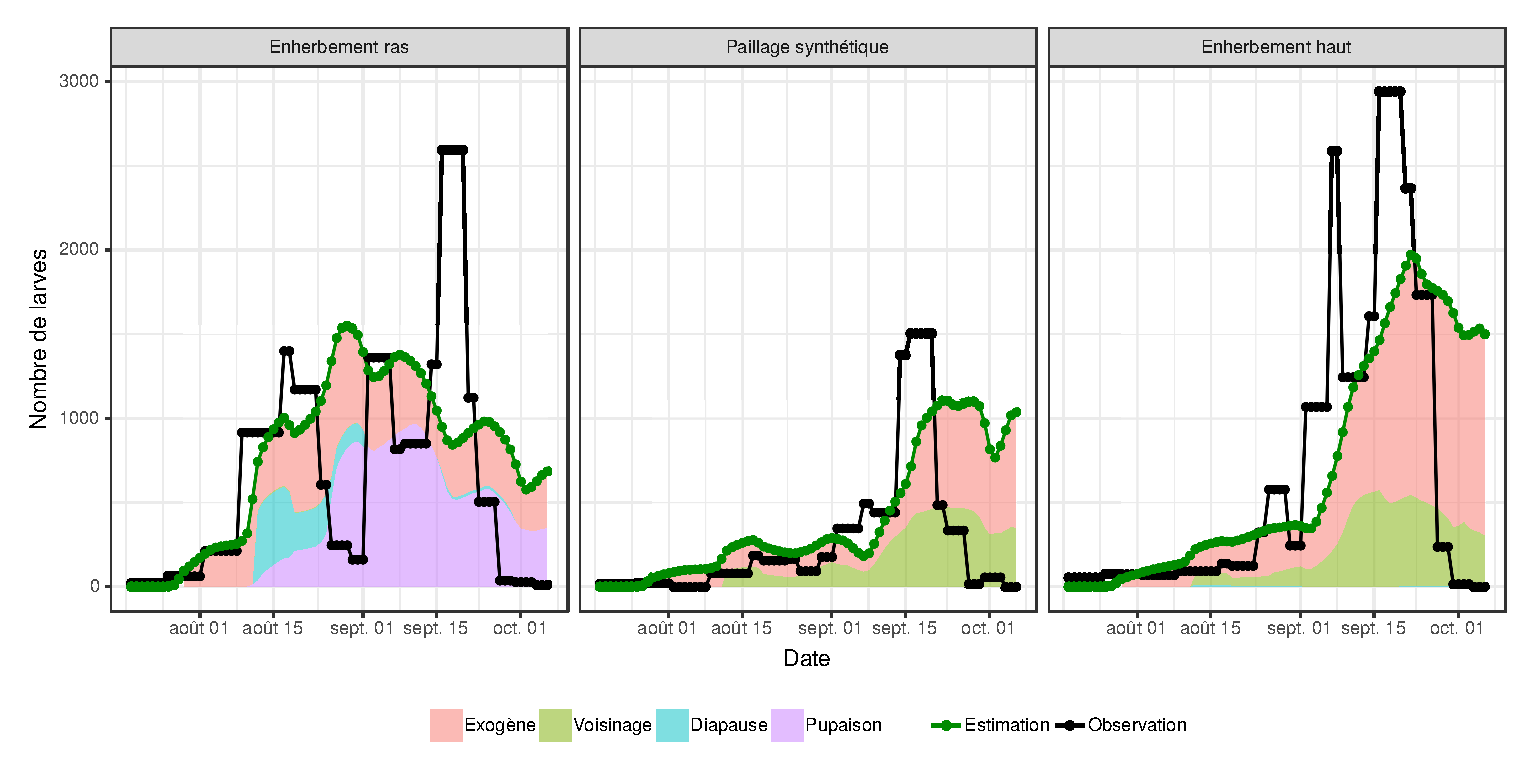
\epsfig{file = A1.eps, scale = 0.2} & 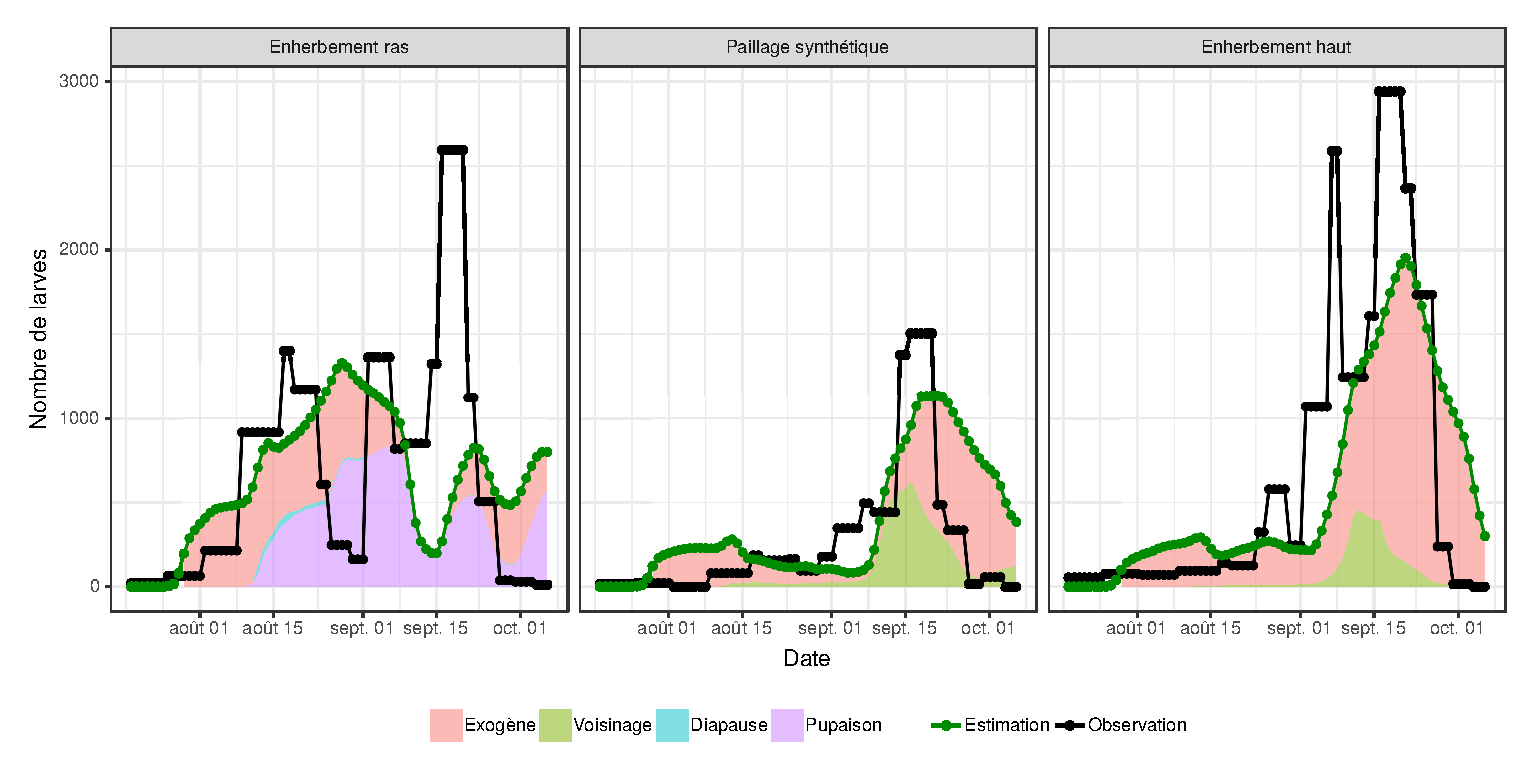
\epsfig{file = C1.eps, scale = 0.2}\\
 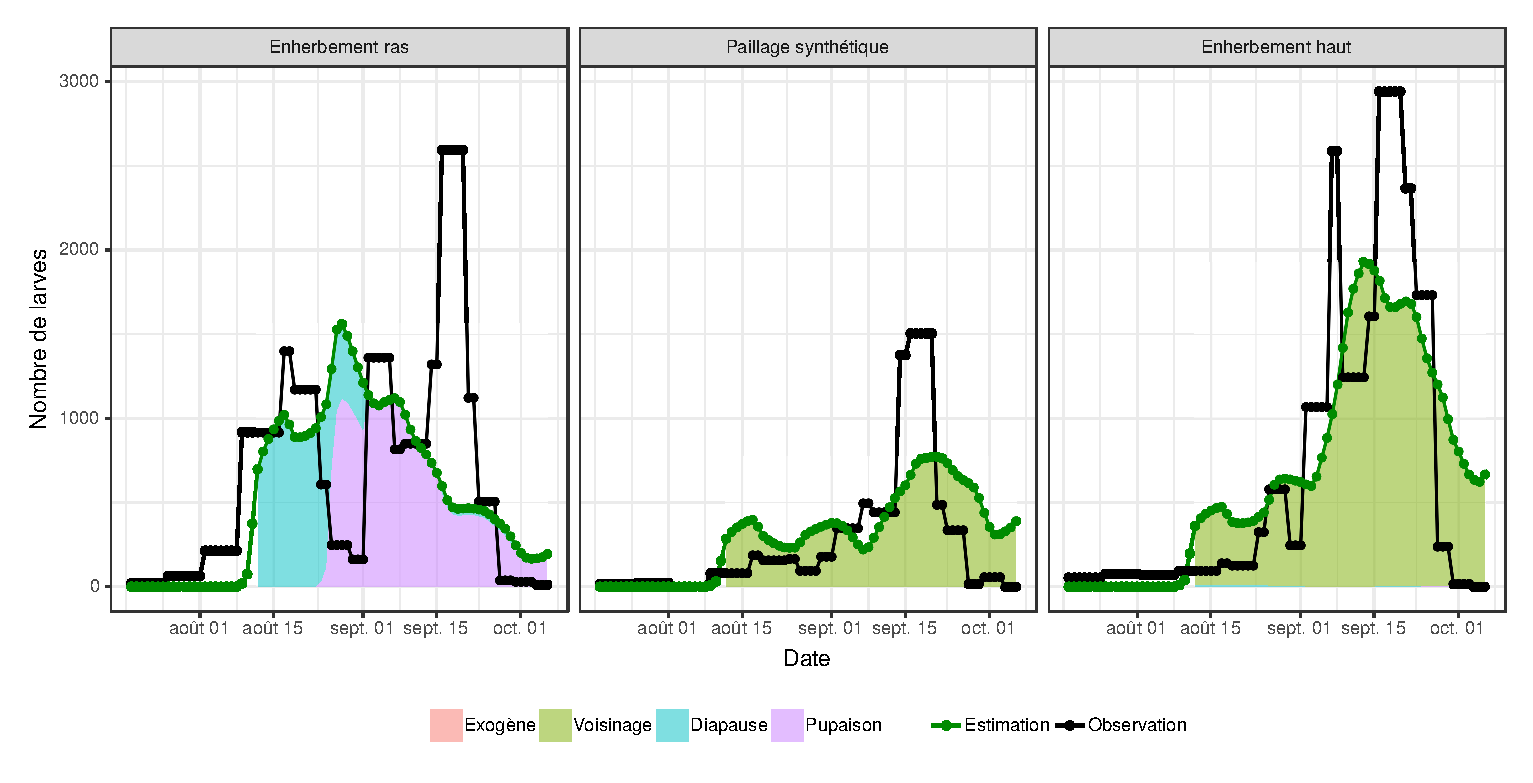
\epsfig{file = A2.eps, scale = 0.2} & 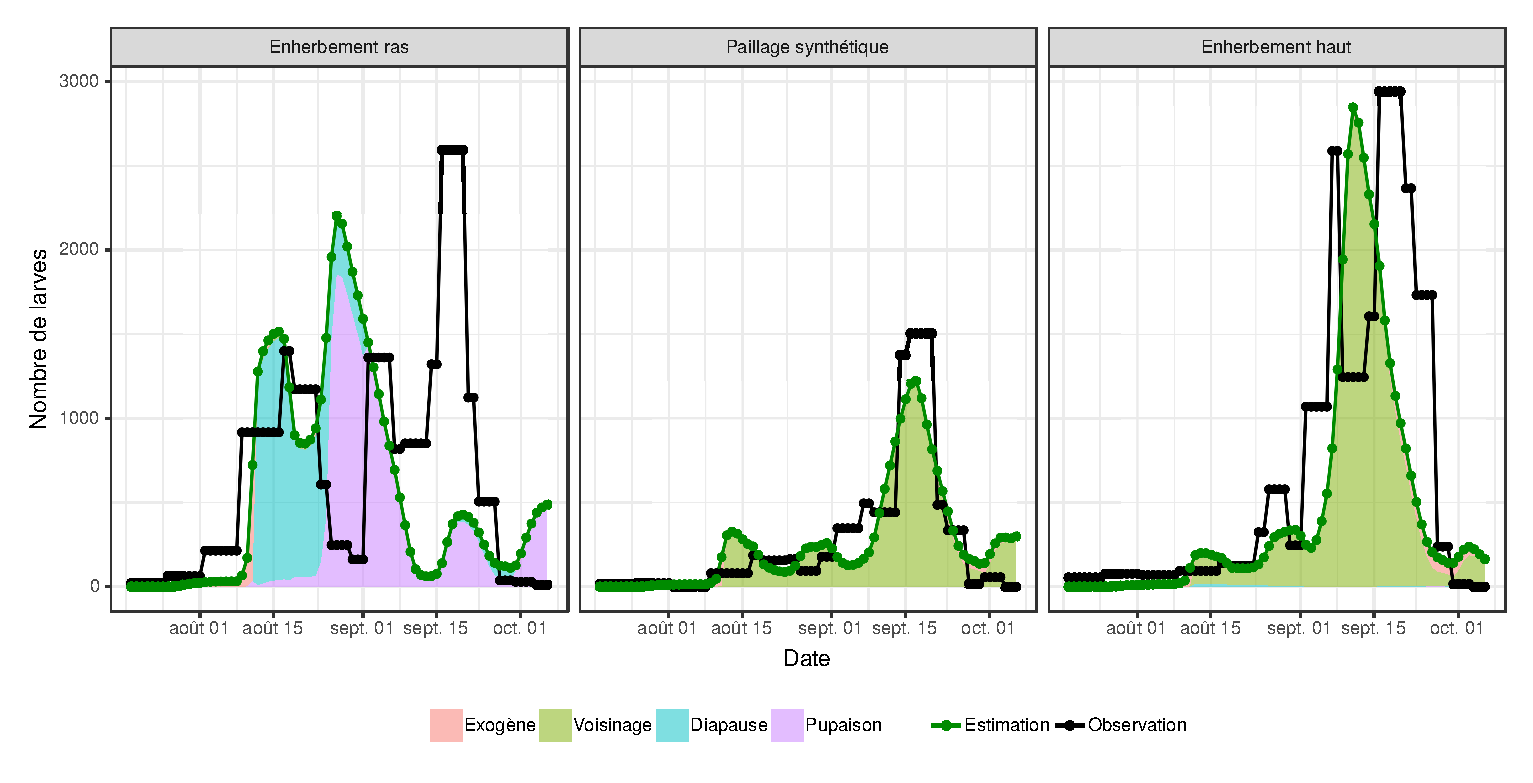
\epsfig{file = C2.eps, scale = 0.2} \\
 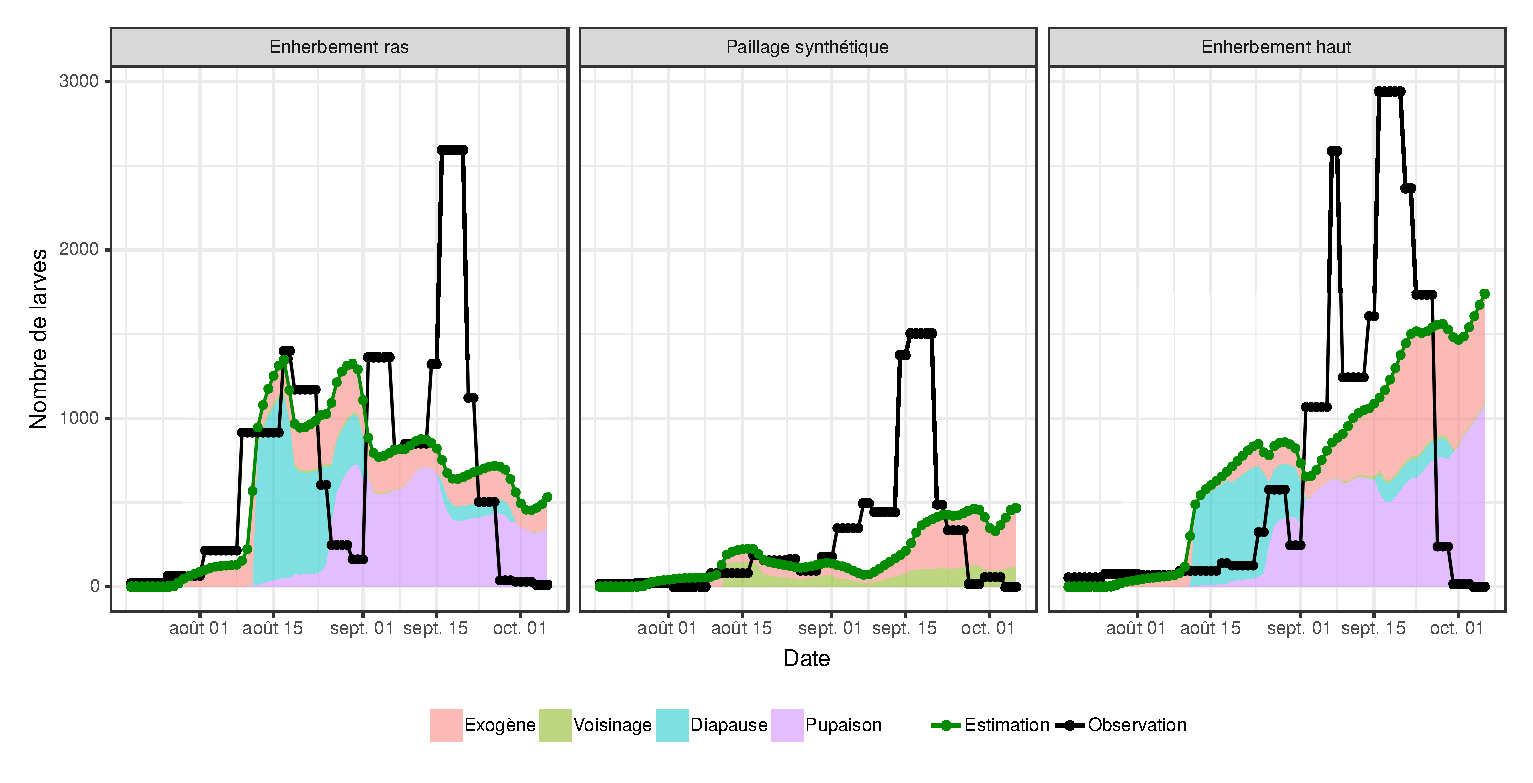
\epsfig{file = A3.eps, scale = 0.2} & 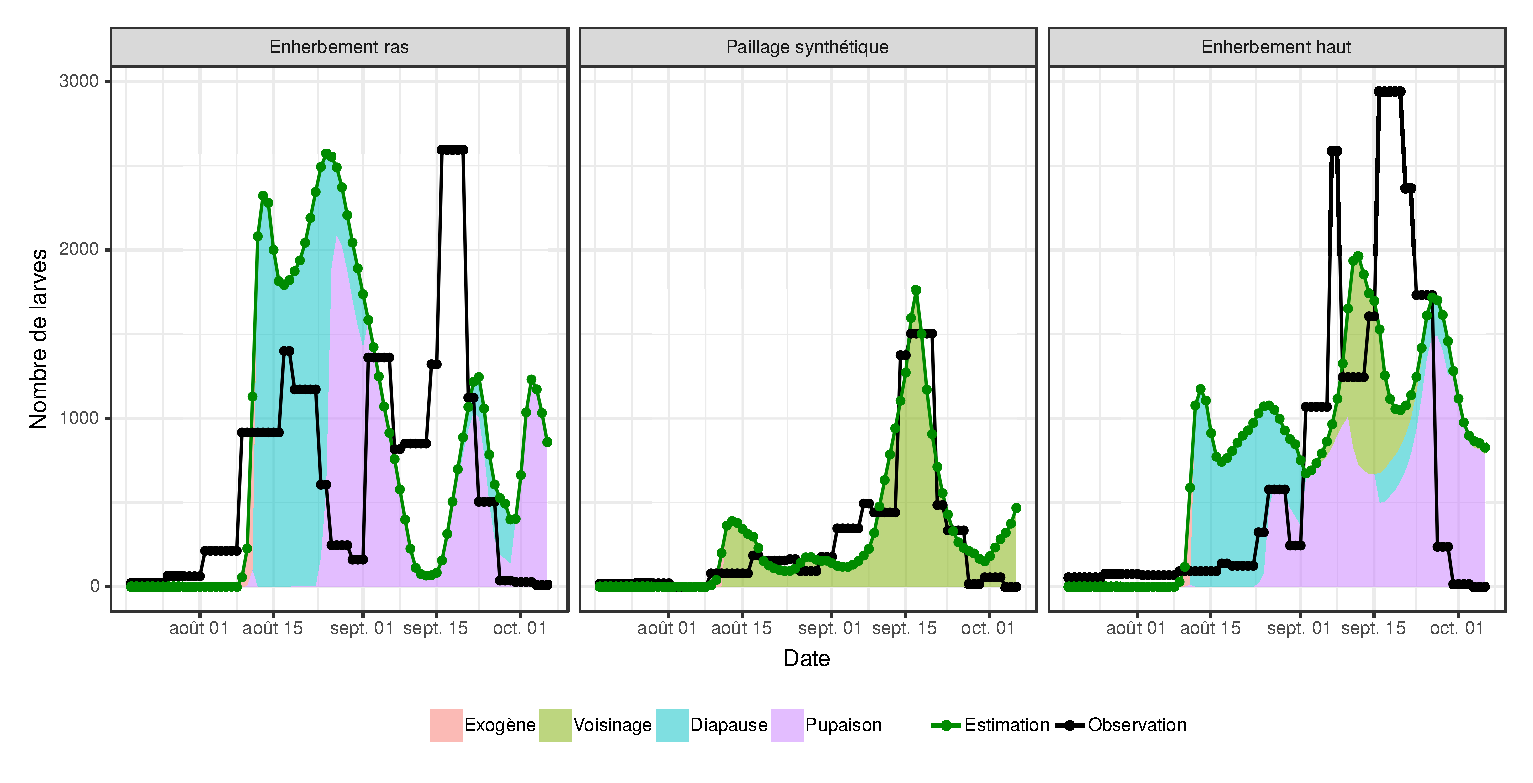
\epsfig{file = C3.eps, scale = 0.2}
\end{tabular}
\end{center}

}
 

 
\end{frame}













\begin{frame}
 \frametitle{Paramètre de saisonnalité}
 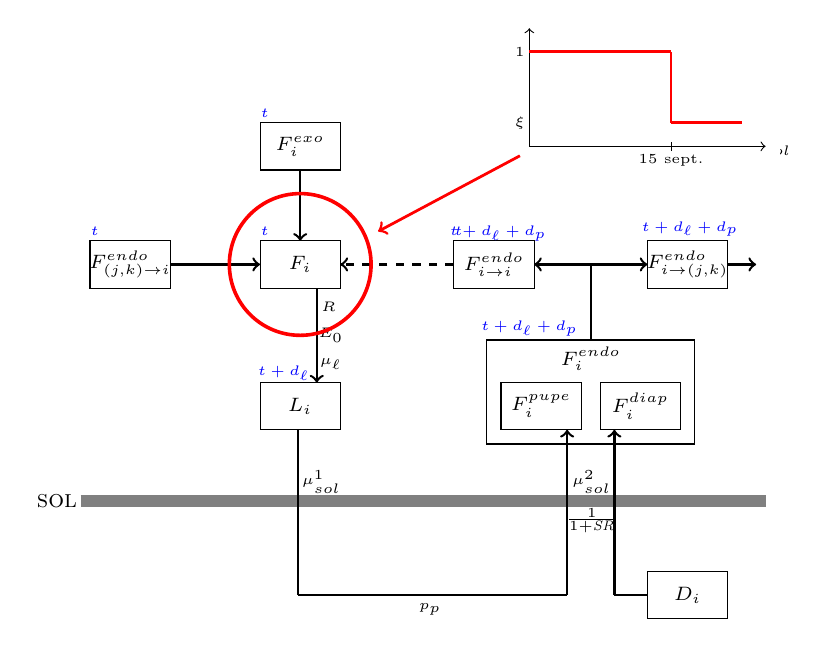
\begin{tikzpicture}[scale = 0.6]
\draw (0, 0) node{\small \textsc{sol}};
\draw [line width = 1.5mm, color = gray] (0.5, 0) -- (15, 0);
   
\draw (4.3,   4.5) rectangle (6, 5.5); % N
\draw (5.15,   5) node {\scriptsize $F_{i}$};
\draw (4.4, 5.7) node {\tiny $\textcolor{blue}{t}$};
% \pause

\draw (4.3,   7) rectangle (6,   8); % N exo
\draw (0.7,   4.5) rectangle (2.4,   5.5); % N voisins
\draw (8.4,   4.5) rectangle (10.1,  5.5); % N endo
\draw (5.15,   7.5) node {\scriptsize $F^\text{exo}_{i}$};
\draw (1.55,  5) node {\scriptsize $F^\text{endo}_{(j,k) \rightarrow i}$};
\draw (9.25,  5) node {\scriptsize $F^\text{endo}_{i\rightarrow i}$};
\draw (0.8, 5.7) node {\tiny $\textcolor{blue}{t}$};
\draw (4.4, 8.2) node {\tiny $\textcolor{blue}{t}$};
\draw (8.5, 5.7) node {\tiny $\textcolor{blue}{t}$};
\draw [->,  line width=0.9] (5.15,   7 ) -- (5.15,  5.5);
\draw [->,  line width=0.9] (2.4,   5 ) -- (4.3,  5);
\draw [->,  line width=0.9] (8.4,   5) -- (6, 5);
%équations
\draw (11, 7.5) node {\scriptsize $F_{t, i} = F^\text{exo}_{t, i} + F^\text{endo}_{t, (j,k) \rightarrow i} + F^\text{endo}_{t, i\rightarrow i}$};
% \pause

\draw (4.3,   1.5) rectangle (6,   2.5); % L
\draw (5.15,   2) node {\scriptsize $L_{i}$};
\draw (4.8, 2.7) node {\tiny $\textcolor{blue}{t + d_{\ell}}$};
\draw (5.75, 4.1)     node {\tiny $R$};
\draw (5.8, 3.5)     node {\tiny $E_0$};
\draw (5.8, 2.9)     node {\tiny $\mu_\ell$};
\draw [->,  line width=0.9] (5.5,  4.5) -- (5.5, 2.5);
\draw [fill = white, white] (7.5, 6.8) rectangle (14.5, 8);
\draw (11, 7.5) node {\scriptsize $L_{t, i} = F_{t-d_\ell, i} \times R \times E_0 \times \mu_\ell$};
% \pause

% \draw (0.7,  -1.5) rectangle (2.4,  -2.5); %diap + mort
\draw (9.4,   1.5) rectangle (11.1,  2.5); % N pupe
% \draw (1.55, -2) node {\scriptsize Exclus};
\draw (10.25, 2) node {\scriptsize $F^{\text{pupe}}_{i}$};
\draw [line width=0.9]     (5.1,   1.5) -- (5.1,  -2);
% \draw [->,  line width=0.9] (5.1,  -2  ) -- (2.4,  -2);
\draw [line width=0.9] (5.1,  -2  ) -- (10.8,  -2);
\draw [->,  line width=0.9] (10.8,  -2 ) -- (10.8,  1.5);
\draw (10, 3.65) node {\tiny $\textcolor{blue}{t + d_{\ell} + d_{\text{p}}}$};
\draw (5.6, 0.4)   node {\tiny $\mu_{\text{sol}}^1$};
\draw (11.32, 0.4) node {\tiny $\mu_{\text{sol}}^2$};
\draw (7.9, -2.3)    node {\tiny $p_{\text{p}}$};
% \draw (3.8, -2.3)    node {\tiny $1-p_{\text{p}}$};
\draw (11.32, -0.42)  node {\tiny $\frac{1}{1 + \mathit{SR}}$};
\draw [fill = white, white] (7.5, 6.8) rectangle (14.5, 8);
\draw (11, 7.5) node {\scriptsize $F^{\text{pupe}}_{t,i} = L_{t-d_{\text{p}}, i} \times \mu_{\text{sol}}^1 \times p_{\text{p}} \times \frac{1}{1 + \mathit{SR}} \times \mu_{\text{sol}}^2$};
% % \pause

\draw (12.5, -1.5) rectangle (14.2, -2.5); %Diap
\draw (13.35,-2) node {\scriptsize $D_{i}$};
\draw (12.35, 2) node {\scriptsize $F^{\text{diap}}_{i}$};
\draw (11.5,  1.5) rectangle (13.2,  2.5); % N diap
\draw [line width=0.9]     (12.5, -2  ) -- (11.8, -2);
\draw [->,  line width=0.9] (11.8,  -2 ) -- (11.8,  1.5);
\draw [fill = white, white] (6.5, 6.8) rectangle (15.3, 8);
\draw (11, 7.5) node {\scriptsize $F^{\text{diap}}_{t,i} = D_{t, i} \times \frac{1}{1+\mathit{SR}} \times \mu_{\text{sol}}^2$};
% \draw (13.4, -1.3) node {\tiny $\textcolor{blue}{t + d_{\ell} + d_{\text{p}}}$};   
% \pause

\draw (9.1,   1.2) rectangle (13.5,  3.4); % N emer
\draw (11.3,  3) node {\scriptsize $F^{\text{endo}}_{i}$};
\draw [fill = white, white] (6.5, 6.8) rectangle (15.3, 8);
\draw (11, 7.5) node {\scriptsize $F^{\text{endo}}_{t,i} = F^{\text{diap}}_{t,i} + F^{\text{pupe}}_{t,i}$};
% \pause

 \draw (12.5,  4.5) rectangle (14.2,  5.5); % N degage

   % TEXTES CASES
\draw (13.35, 5) node {\scriptsize $F^\text{endo}_{i\rightarrow (j,k)}$};
% \draw (13, -1.3) node {\tiny $\textcolor{blue}{t + d_{\ell}}$};   
\draw (9.34, 5.65) node { \tiny $\textcolor{blue}{t + d_{\ell} + d_{\text{p}}}$};
\draw (13.4, 5.75) node {\tiny $\textcolor{blue}{t + d_{\ell} + d_{\text{p}}}$};
\draw [line width=0.9]     (10.1, -2  ) -- (10.8, -2);
\draw [line width=0.9]     (11.3,  3.4) -- (11.3,  5);
\draw [->,  line width=0.9] (11.3,   5 ) -- (10.1,  5);
\draw [->,  line width=0.9] (11.3,   5 ) -- (12.5,  5);
\draw [->,  line width=0.9] (14.2,   5 ) -- (14.8,  5);
\draw [fill = white, white] (6.5, 6.8) rectangle (15.3, 8);
\draw [fill = white, white] (6.05, 4) rectangle (8.35, 5.5);
\draw [->,  line width=0.9, dashed] (8.4,   5) -- (6, 5);
% \draw (11, 7.5) node {\scriptsize $F_{t, i \rightarrow j}^{\text{endo}} = \frac{I_{t, j} \times p_{\text{m}}^{\delta(i, j)}}{\sum_{n\in \{i,j,k\}} I_{t, n} \times p_{\text{m}}^{\delta(i, n)}}\times F_{t, i}^{\text{endo}}$};
% \draw [->, line width = 1.3, color = red] (9, 7.5) -- (6, 7.5);
% \draw [->, line width = 1.3, color = red] (3, 4.1) -- (5.5, 4.1);
\draw [line width = 1.3, color = red] (5.15, 5) circle (1.5);

\draw [->] (10, 7.5) -- (10, 10);
\draw [->] (10, 7.5) -- (15, 7.5);
\draw [red, line width = 1] (10, 9.5) -- (13, 9.5);
\draw [red, line width = 1] (13, 9.5) -- (13, 8);
\draw [red, line width = 1] (13, 8) -- (14.5, 8);
\draw (9.8, 9.5) node {\tiny 1};
\draw (9.8, 8) node {\tiny $\xi$};
\draw (13, 7.2) node {\tiny 15 sept.};
\draw (13, 7.4) -- (13, 7.6);
\draw [->, red, line width =1] (9.8, 7.3) -- (6.8, 5.7);
\end{tikzpicture}
\end{frame}

















%% SOLUTIONS 2
\begin{frame}
 \frametitle{Paramètre de saisonnalité}
 
 
 
 
 \begin{figure}
  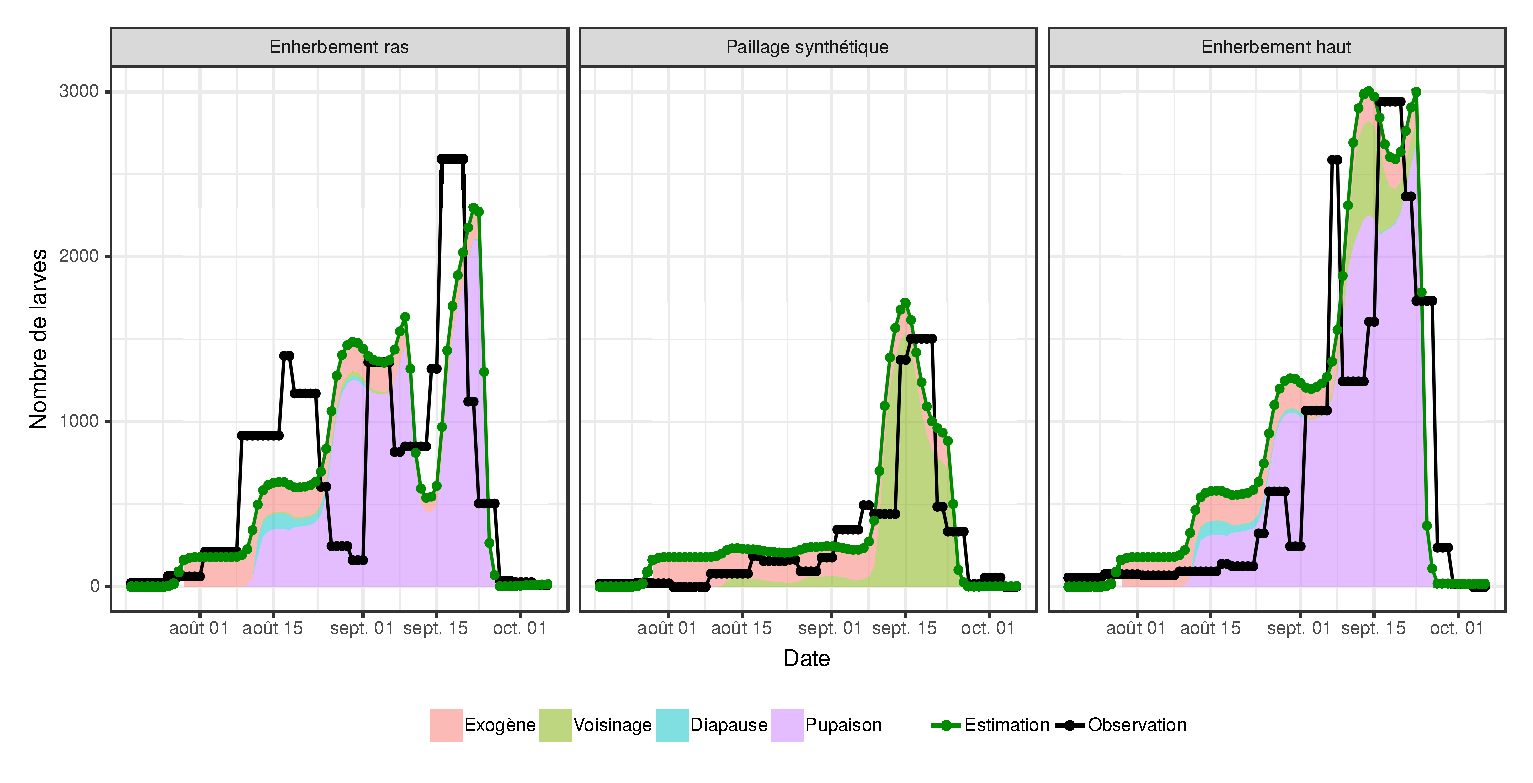
\epsfig{file = D1.eps, scale = 0.3}
 \end{figure}

 \pause
 \begin{figure}
  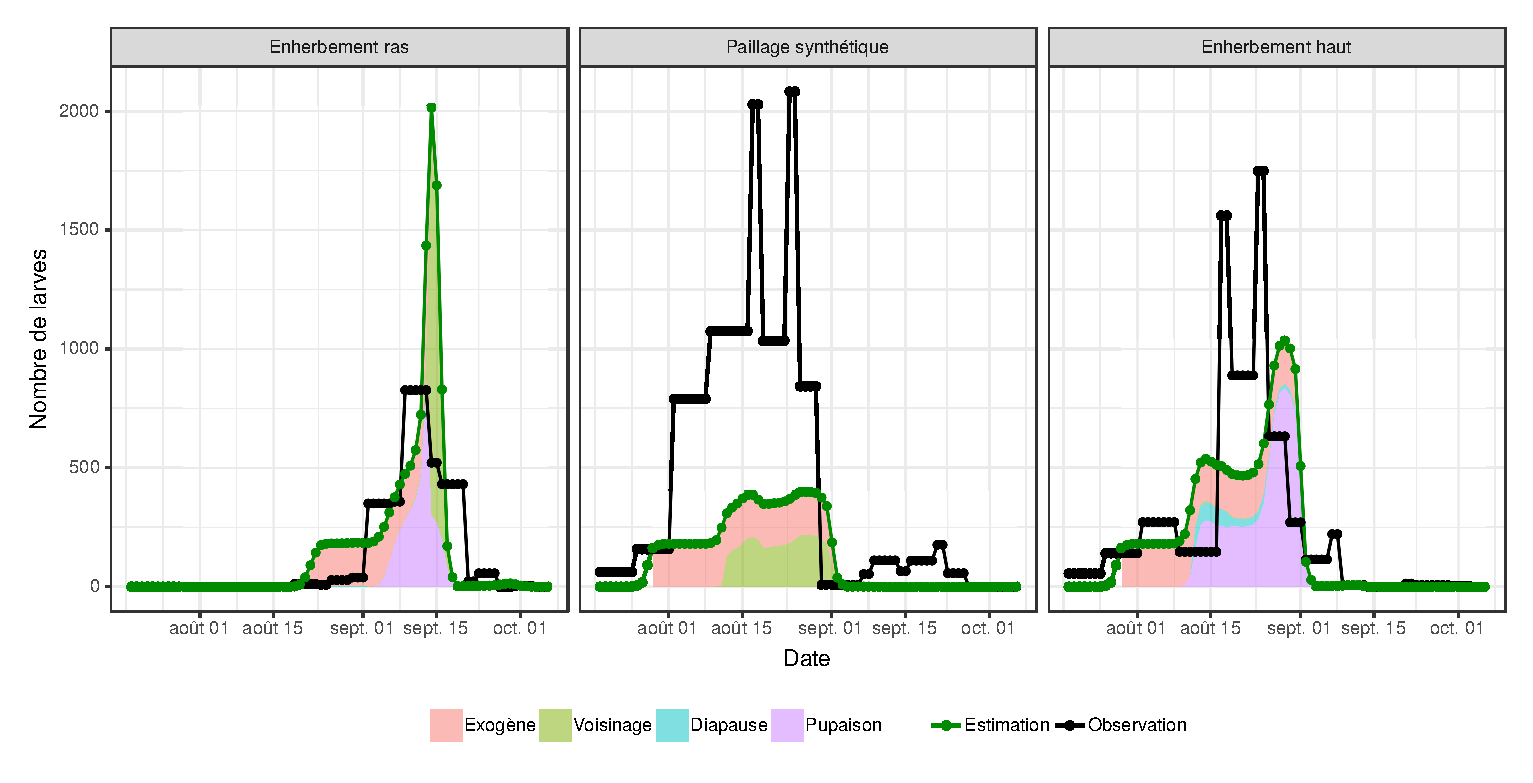
\epsfig{file = D_b2.eps, scale = 0.3}
 \end{figure}

 
\end{frame}


















%% CONCLUSION
\begin{frame}
 \frametitle{Conclusion}
 
À partir des connaissances issues de la littérature et de données acquises sur le terrain, un modèle a pu être établi.

\vspace{1cm}

Le modèle a permi de tester des hypothèses.

\vspace{1cm}

Le modèle semble montrer qu'un phénomène se produit en fin de saison.

\vspace{1cm}

Perspectives pour de nouvelles expérimentations

\end{frame}


















%% MERCI
\begin{frame}

{\color{bleu} Merci de votre attention !}
\end{frame}















\end{document}
